\documentclass[11pt,a4paper]{report}

\usepackage{fancyhdr}
\usepackage{}
\usepackage{amssymb}
\usepackage{amsmath}
\usepackage{graphicx}
\usepackage[T1]{fontenc}
\usepackage{hyperref}
\hypersetup{colorlinks=true,linkcolor=cyan, citecolor=green,filecolor=black,urlcolor=blue}
\usepackage{epstopdf}
\usepackage{makeidx}
\usepackage{tocloft}
\usepackage{tikz}
\usetikzlibrary{shapes,shadows,arrows}

\tikzstyle{startstop} = [rectangle, rounded corners, minimum width=2cm, minimum height=1cm,text centered, draw=black, fill=red!30]
\tikzstyle{io} = [trapezium, trapezium left angle=70, trapezium right angle=110, minimum width=3cm, minimum height=1cm, text centered, draw=black, fill=blue!30]
\tikzstyle{process} = [rectangle, minimum width=5cm, minimum height=1cm, text centered, text width=5cm, draw=black, fill=orange!30]
\tikzstyle{decision} = [diamond, minimum width=3cm, minimum height=1cm, text centered, draw=black, fill=green!30]
\renewcommand{\headrulewidth}{0pt}
\renewcommand{\footrulewidth}{0pt}
\renewcommand{\cftchapleader}{\cftdotfill{\cftdotsep}}
\renewcommand{\contentsname}{Cuprins}
\renewcommand{\bibname}{B\lowercase{ibliografie}}
\renewcommand{\chaptername}{Capitolul}
\renewcommand{\appendixname}{Anexa}
\renewcommand{\indexname}{I\lowercase{indice}}
\pagestyle{fancy}
\makeindex
\newtheorem{prop}{Propozi\c tie}
\newenvironment{demo}{\paragraph{\textbf{Demonstra\c{t}ie}:}}{\hfill$\square$}
\newcommand{\R}{\mathbb{R}}
\tikzstyle{arrow}=[thick,-,>=stealth]
\begin{document}
	\pagenumbering{roman}
	

\begin{titlepage}
	\begin{center}
		\large
		\textsc{Universitatea ,\hspace{-0.02cm},Alexandru Ioan Cuza'', Ia\c si}\\
		\textsc{Facultatea de Matematic\u{a}}\\[0.3cm]
 		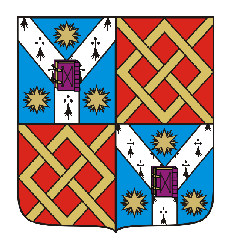
\includegraphics[scale=.4]{stema.eps}
		\vfill
		
		%Titlu
		\Huge
		\textsc{Algoritmi pentru grafuri \c si aplica\c{t}ii}\\[0.8cm]
		\large
		\textbf{Lucrare de licen\c t\u a}
		
		\vfill
		\begin{minipage}[t]{0.49\textwidth}
			\begin{flushleft}
				\large
				\textbf{Conduc\u{a}tor \c{s}tiin\c{t}ific:}\\
				Lect.Dr. Ana-Maria Mo\c{s}neagu
			\end{flushleft}
		\end{minipage}
	    \hfill
	    \begin{minipage}[t]{0.49\textwidth}
	    	\begin{flushright}
	    		\large
	    		\textbf{Student:}\\
	    		Galbini\c t\u a Sebastian
	    	\end{flushright}
    	\end{minipage}
	    
	    \vfill
	    \large
	    \centering
	    Septembrie, 2020\\
	    Ia\c{s}i
	\end{center}
\end{titlepage}

	\thispagestyle{empty}
	\pdfbookmark[1]{Cuprins}{Cuprins}
	\tableofcontents
	\thispagestyle{empty}
	\fancyhf{}
		\clearpage
    \pagenumbering{arabic}

	
	\chapter*{Introducere}
	\addcontentsline{toc}{chapter}{Introducere}	
	Multe aplica\c tii computa\c tionale invoc\u a nu numai o pereche de obiecte dar \c si un set de conexiuni care s\u a lege aceste informa\c tii \^intre ele. Rela\c tia impus\u a dintre aceste conexiuni a condus la mai multe \^intreb\u ari precum: Exist\u a posibilitatea s\u a ajungi de la un obiect la altul urm\u arind conexiunile? La c\^ ate obiecte pot s\u a ajung pornind de la unul deja prestabilit? Care ar fi cel mai scurt/lung drum parcurs pentru a ajunge la destina\c tia propus\u a? Exist\u a o leg\u atur\u a \^ intre toate tipurile de date? Pentru a ilustra diversitatea aplica\c tiilor ce folosesc propriet\u a\c ti \c si metode, care au ca fundament grafurile, enumer\u am urm\u atoarele exemple: H\u ar\c tile, Hypertexts (documente ce con\c tin referin\c te c\u atre alte pagini web), Circuite, Tranzac\c tii, Re\c tea de internet etc.
	
	Pentru a putea r\u aspunde la \^ intreb\u arile de mai sus, vom folosi obiecte abstracte cum ar fi grafurile. Grafurile sunt structuri de date extrem de r\u asp\^ andite \^ in \c stiin\c ta calculatoarelor, iar algoritmii pentru grafuri sunt esen\c tiali \^ in acest domeniu.
	
	\^ In capitolul 1 sunt prezentate c\^ ateva no\c tiuni introductive legate de grafuri, cum ar fi: reprezentarea grafurilor pe calculator, no\c tiunea de grad \c si drum  \c si aspecte legate de conexitatea unui graf.
	
	\^ In  capitolul 2 se trateaz\u a problema de   determinare a drumurilor de lungime minim\u a de la un nod fixat la toate celelalte noduri, atunci c\^ and fiec\u arei muchii \^ ii este  asociat\u a o lungime pozitiv\u a. Se va prezenta algoritmul de relaxare aplicat unei muchii iar la final se va descrie \c si implementa algoritmul lui Dijkstra pentru problema de drum minim.
	
	\^ In capitolul 3 se va rezolva problema  determin\u arii a tuturor drumurilor de cost minim \^ intre oricare dou\u a noduri. Pentru determinarea unei solu\c tii optime se va studia structura unui drum minim \c si se vor prezenta  algoritmii necesari pentru rezolvarea acestei probleme.
		
	\^ In final, \^ in capitolul 4 se va rezolva problema de flux maxim care se refer\u a la determinarea  celei mai mari cantit\u a\c ti de material care poate fi transportat\u a de la surs\u a la destina\c tie \c tin\^ and cont de restric\c tiile de capacitate \^ intr-un graf orientat ponderat. Definim formal problema fluxului maxim, no\c tiunile de re\c tea de transport \c si flux de re\c tea iar la final se va descrie metoda lui Ford-Fulkerson pentru g\u asirea fluxului maxim.
	
	
	

	\chapter{No\c tiuni introductive}
	
	\section{Graf}
	
    Un \textit{graf} $G=(V,E)$ este o pereche  de mul\c timi astfel \^ inc\^ at $E\subseteq V\times V$. Elementele din mul\c timea $V$ se numesc \textit{noduri} ale grafului $G$ iar elementele mul\c timii $E$ se numesc \textit{muchii}. Modul obi\c snuit de a ilustra un graf este prin desenarea unui punct pentru fiecare nod \c si unirea celor dou\u a puncte printr-o linie, dac\u a cele dou\u a v\^ arfuri corespunz\u atoare formeaz\u a o muchie.
	
	
	\begin{figure}[!hbt]
		\centering
		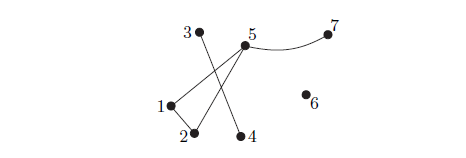
\includegraphics[width=10.2cm]{Figura1.png}
		\caption{Graful pe $V=\{ 1,2,3,...,7\}$ cu setul de muchii \centering \newline $E=\{ \{1,2\},\{1,5\},\{2,5\},\{3,4\},\{5,7\} \}$ }
		\end{figure}
	
	Se spune c\u a un graf cu setul de noduri $V$ este un graf pe $V$. Setul de noduri al unui graf $G$ este notat cu $V(G)$, muchiile sale fiind $E(G)$. Aceste conven\c tii sunt independente de orice alte denumiri ale acestor dou\u a seturi: setul de noduri $W$ a grafului $H=(W,F)$ este tot notat prin $V(H)$, nu prin $W(H)$. Num\u arul de noduri ale unui graf $G$ d\u a \textit{ordinul} acestuia, notat prin $|G|$; num\u arul s\u au de muchii este notat cu $||G||$. Grafurile pot fi de ordin \textit{finit}, \textit{infinit} sau \textit{num\u arabil}. Pentru \textit{graful null} $(\emptyset,\emptyset)$ scriem pur \c si simplu $\emptyset$. Un graf de ordin 0 sau 1 se nume\c ste \textit{trivial}.
	
	Un nod $v$ este \textit{incident} cu o muchie $e$ dac\u a $v\in e$; atunci $e$ este o muchie la $v$. O muchie $\{u,v\}$ este de obicei scris\u a sub forma $(u,v)$. V\^ arfurile $u$ \c si $v$ se numesc \textit{extremit\u a\c tile muchiei} $(u,v)$. 
	
	Dou\u a noduri ale grafului $G$ sunt \textit{adiacente} sau \textit{vecine} dac\u a $(x,y)$ formeaz\u a o muchie pe $G$. Dou\u a muchii care au o extremitate comun\u a, se numesc \textit{muchii incidente}. Dac\u a toate v\^ arfurile lui $G$ sunt perechi adiacente, atunci $G$ este \textit{complet}. 
	
	Fie $G=(V,E)$ \c si $G'=(V',E')$ dou\u a grafuri. Numim $G$  \c si  $G'$  \textbf{izomorfe} \c si not\u am $G\simeq G'$ dac\u a exist\u a o bijec\c tie $\varphi :V\rightarrow V'$ cu $(x,y)\in E  \Leftrightarrow (\varphi (x),\varphi (y)) \in E'$ pentru orice $x,y\in V$.
	
	\begin{figure}[!hbt]
		\centering
		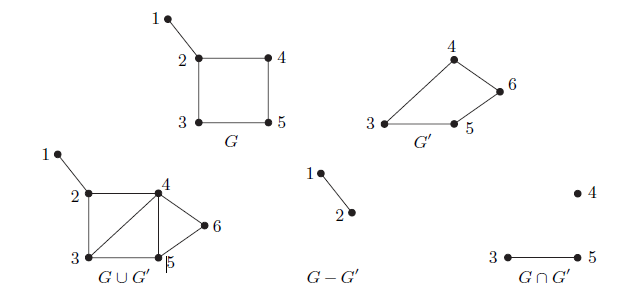
\includegraphics[width=12.2cm]{Figura2.png}
		\caption{Reuniunea, diferen\c ta \c si intersec\c tia; v\^ arfurile 2,3,4 \centering \newline formeaz\u a un triunghi \^ in $G\cup G'$ dar nu \^ in $G$}
	\end{figure}
	
	
	Stabilim c\u a $G\cup G'=(V\cup V',E\cup E')$ \c si $G\cap G'=(V\cap V',E\cap E')$. Dac\u a $G\cap G'=\emptyset$, atunci $G$ \c si $G'$ sunt \textit{disjuncte}. Dac\u a $V'\subseteq V$ \c si $E'\subseteq E$, atunci $G'$ este un \textit{subgraf} al lui $G$ (\c si $G$ este un \textit{supergraf} pentru $G'$), scris ca $G'\subseteq G$. Mai pu\c tin formal, spunem c\u a $G$ \^ il con\c tine pe $G'$.
	 
    \section{Reprezentarea unui graf}
	Un \textit{graf neorientat} \cite{AM} $G$ este o pereche $(V,E)$, unde $V$ reprezint\u a o mul\c time finit\u a numit\u a \textit{mul\c timea nodurilor} lui $G$, iar $E$ este o mul\c time de perechi neordonate $(u,v)\in V\times V$, numit\u a \textit{mul\c timea muchiilor} lui $G$. Prin urmare, fiecare muchie este o pereche neordonat\u a de noduri $(u,v)\in E$, prin care este stabilit\u a o rela\c tie de vecin\u atate \^ intre $u,v\in V$. Figura 1.3(a) este o reprezentare grafic\u a a unui graf neorientat.

\^ Intr-un \textit{graf orientat} \cite{AM} $G=(V,E)$, \textit{mul\c timea arcelor} $E$ este constituit\u a din perechi de v\^ arfuri ordonate \c si nu din perechi neordonate. Arcul $(u,v)\in E$ este reprezentat printr-o s\u ageat\u a de la nodul $u$ la $v$ cu semnifica\c tia c\u a exist\u a o rela\c tie de la $u$ la $v$. Figura 1.4(a) este o reprezentare grafic\u a a unui graf orientat.   
   
    Exist\u a dou\u a moduri de reprezentare a unui graf $G=(V,E)$: ca o colec\c tie de liste de adiacen\c t\u a sau ca o matrice de adiacen\c t\u a. Oricare dintre aceste dou\u a  modalit\u a\c ti de reprezentare, se aplic\u a at\^ at grafurilor orientate c\^ at \c si celor neorientate.
    
    \textbf{Reprezentarea prin liste de adiacen\c t\u a} \cite{Cormen} a grafului $G=(V,E)$ const\u a \^ in realizarea unui tablou $M$ cu |V| liste, o list\u a pentru fiecare v\^ arf din $V$. Pentru fiecare $u\in V$, $M[u]$ con\c tine toate v\^ arfurile $v$ astfel \^ inc\^ at exist\u a o muchie $(u,v)\in E$. Figura 1.3(b) este o reprezentare prin liste de adiacen\c t\u a a grafului neorientat din Figura 1.3(a). At\^ at pentru grafurile orientate c\^ at \c si pentru cele neorientate, reprezentarea lor prin liste de adiacen\c t\u a au o dimensiunea de memorie de $O(V+E)$.
    
    Listele de adiacen\c t\u a pot fi adaptate \c si pentru reprezentarea unor \textbf{grafuri ponderate} astfel, fiecarei muchii a grafului $G$ i se asociaz\u a o func\c tie numit\u a \textbf{func\c tie de cost} $f :E\to \R $, unde costul $f(u,v)$ al muchiei $(u,v)$ este memorat \^ impreun\u a cu $v$ \^ in $M[u]$. 
    
    \^ In majoriatea cazurilor, listele de adiacen\c t\u a se folosesc atunci c\^ and vrem s\u a gestion\u am memoria programului c\^ at mai eficient. De exemplu, dac\u a avem un graf \textit{rar} ($|E|$ este mult mai mic dec\^ at $|V|(|V|-1)/2$) \c si am folosi reprezentarea grafului cu ajutorul matricelor, atunci majoritatea elementelor din matrice ar r\u am\^ ane nefolosite, produc\^ and astfel o risip\u a de memorie.
    	\begin{figure}[!hbt]
    	\centering
    	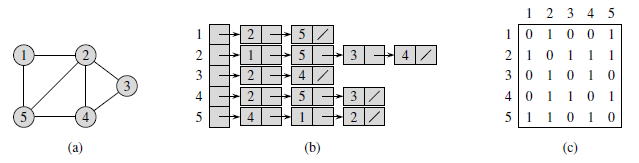
\includegraphics[width=13.2cm]{Figura4.png}
    	\caption{Dou\u a reprezent\u ari a unui graf neorientat.(\textbf{a}) Graf  neorientat. \centering \newline(\textbf{b}) List\u a de adiacen\c t\u a pentru $G$.(\textbf{c}) Matricea de adiacen\c t\u a a lui $G$.}
    \end{figure}

    \begin{figure}[!hbt]
	\centering
	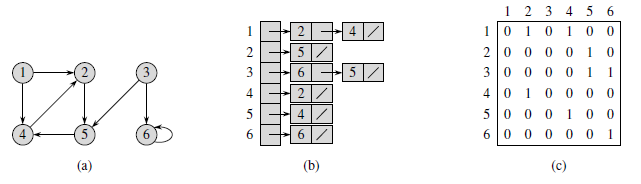
\includegraphics[width=13.2cm]{Figura5.png}
	\caption{Dou\u a reprezent\u ari a unui graf orientat.(\textbf{a}) Graf orientat. \centering \newline(\textbf{b}) List\u a de adiacen\c t\u a pentru $G$.(\textbf{c}) Matricea de adiacen\c t\u a a lui $G$.}
    \end{figure}
    
    
    Pentru \textbf{reprezentarea prin matrice de adiacen\c t\u a} \cite{Cormen}, presupunem c\u a v\^ arfurile sunt numerotate arbitrar. Reprezentarea matricii de adiacen\c t\u a a grafului $G=(V,E)$ const\u a \^ intr-o matrice $A_{|V|\times |V|}=(a_{ij})$ a.\^ i.:
    \begin{equation*}
    a_{ij}=\begin{cases}
    1, (i,j)\in E \medskip \\
    0, (i,j)\notin E
    \end{cases}
    \end{equation*}
    
    Figuriele 1.3(c) \c si 1.4(c) sunt reprezent\u arile matricilor de adiacen\c t\u a a grafurilor 1.3(a), respectiv 1.4(a). Necesarul de memorie este de $\Theta(|V|^2)$ \c si nu depinde de num\u arul de muchii a grafului. \^ In plus, c\^ and se face implementarea cu ajutorul matricelor, verificarea dac\u a este o muchie \^ intre cele dou\u a v\^ arfuri dureaz\u a $\Theta(1)$ timpi, \^ in timp ce cu ajutorul listelor de adiacen\c t\u a ar putea avea un ordin de complexitate liniar $\Theta(n)$, unde $n$ este  num\u arul de noduri.
    
     Matricile de adiacen\c t\u a pot fi folosite \c si pentru grafuri ponderate. Astfel, fie un graf orientat ponderat $G=(V,E)$ \c si func\c tia de cost $f$ de mai sus. Costul $f(u,v)$ al unei muchii $(u,v)\in E$ este memorat ca un element din matrice. \^ In cazul \^ in care o muchie nu exist\u a, elementul corespunz\u ator din matrice poate fi $NIL$.
    
    Un avantaj pentru folosirea matricilor \^ in locul listelor este acela c\u a dac\u a graful este \textit{dens} ($|E|$ este aproximativ egal cu  $|V|^2$) atunci num\u arul de muchii este aproape de $n(n-1)/2$ , unde $n=|V|$.
    \section{Gradul unui nod}
    
    
    Fie $G=(V,E)$ un graf neorientat nenul. Mul\c timea vecinilor nodului  $v$ \^ in $G$ este notat\u a cu $N_G(v)$ sau pe scurt $N(v)$. Mai general, pentru $U\subseteq V$, vecinii din $V\setminus U$ ai nodurilor din $U$ se numesc vecini lui $U$; mul\c timea lor este notat\u a cu $N(U)$.
    
    \textbf{Gradul} $d_G(v)=d(v)$ a unui nod $v$  este num\u arul de muchii $|E|$ la $v$. Dac\u a gradul unui nod este $0$ atunci acesta se nume\c ste \textit{nod izolat}. Num\u arul $\delta(G)=min\, \{\,d(v)\, |\, v\in V\, \}$ este \textit{gradul minim} \cite{Bondy} a lui $G$, iar num\u arul $\Delta(G)=max\, \{\, d(v)\, |\, v\in V\,\}$ este \textit{gradul maxim} \cite{Bondy} a lui $G$. Dac\u a toate nodurile lui $G$ au acela\c si grad $k$, atunci $G$ este \textit{k-regulat}, sau simplu \textit{regulat}. Un graf 3-regulat se nume\c ste \textit{cub}.
    
    Num\u arul
        \begin{equation*}
    d(G)=\frac{1}{|V|} \sum\limits_{v\in V} d(v)
    \end{equation*}
    se nume\c ste \textit{gradul mediu } \cite{Bondy} a lui $G$. Deasemena, are loc rela\c tia,
    \begin{equation*}
    \delta(G)\le d(G)\le \Delta(G)
    \end{equation*}
    
    
    
    \section{Drumuri si cicluri}
    \textbf{Drumul} este un graf orientat nenul $=(V,E)$ de forma 
    \begin{equation*}
    V=\{v_1,v_2,...,v_k\}\quad E=\{(v_0,v_1),(v_1,v_2),...,(v_{k-1},v_k)\}
    \end{equation*}
    unde toate nodurile $v_i$ sunt distincte. Num\u arul de muchii a unui drum reprezint\u a \textit{lungimea } lui. Un \textit{drum elementar} este un drum \^ in care nodurile sunt distincte dou\u a c\^ ate dou\u a.
    
    Fiind date dou\u a mul\c timi $A,B$ de noduri, spunem c\u a $P=[\,x_0,x_1,...,x_k\,]$ este un \textit{drum A-B} dac\u a $V(P)\cap A=\{x_0\}$ \c si $V(P)\cap B=\{x_k\}$. Dou\u a sau mai multe drumuri sunt \textit{independente} dac\u a nici unul dintre ele nu con\c tine un nod interior al altuia.
    
    Dac\u a $P=[\,x_0,x_1,...,x_{k-1}\,]$ este un drum \c si $k\ge 3$, atunci graful $C=P+(x_{k-1},x_0)$ este un \textit{ciclu}. Ca \c si la drumuri, vom nota ciclul dup\u a secven\c ta de noduri pe care o are; ciclul de mai sus $C$ poate fi scris  sub forma $C=[\,x_0,...,x_{k-1},x_0\,]$.
    
    \textit{Distan\c ta} dintre dou\u a noduri \^ in $G$, $d_G(x,y)$ este lungimea celui mai scurt drum $x-y$ \^ in $G$; dac\u a nu exist\u a un astfel de drum vom nota $d(x,y)=\infty$. Cea mai mare distan\c t\u a dintre oricare dou\u a noduri \^ in $G$ este \textit{diametrul} lui $G$, notat\u a cu $diam\,\,G$.
    
   %% \begin{prop}
    %%	Orice graf $G$ de con\c tine un drum de lungime $\delta(G)$ si un ciclu de lungime m\u acar $\delta(G)+1$(numai pentru $\delta(G)\ge 2$)
     %%\end{prop}
    %%\begin{demo}
    %%	Fie $x_1,...,x_k$ cel mai lung drum al lui $G$, care nu poate fi extins. Orice vecin a lui $x_1$ trebuie s\u a fie pe drum, deoarece %%altfel am putea s\u a o extindem. \^ Intruc\^ at $x_1$ are m\u acar $\delta (G)$ vecini, atunci mul\c timea $\{x_2,x_3,...,x_k\}$ trebuie %%s\u a con\c tin\u a $\delta (G)$ elemente. Prin urmare $k\ge \delta (G)+1$, are lungimea drumului de cel pu\c tin $\delta (G)$.
    %%\end{demo}
    \section{Conexitate}
    
    Un graf neorientat nenul $G=(V,E)$ se nume\c ste \textbf{conex} dac\u a pentru orice $u,v\in V $, $u\neq v$ exist\u a cel pu\c tin un drum de la $u$ la $v$. Un subgraf maximal conex la $G$  se nume\c ste \textit{component\u a conex\u a} la $G$. Mai general, pentru orice subgraf $S=(V_1,E_1)$ la $G$, $S$ este convex \c si nu exist\u a un alt subgraf la $G$, $S'=(V_2,E_2)$ cu $V_1\subset V_2$ care s\u a fie conex. Un graf cu un singur nod este graf conex.
    
    Pentru grafurile orientate, vom eviden\c tia dou\u a no\c tiuni asociate cu no\c tiunea de conexitate. 
    Un graf orientat se numește \textit{slab conex} \cite{AM} dacă înlocuirea tuturor muchiilor orientate, cu muchii ale unui graf neorientat produce un graf conex (neorientat). Un graf orientat este \textit{tare conex} \cite{AM} dac\u a oricare ar fi dou\u a noduri $u,v\in E$, exist\u a drum \c si de la $u$ la $v$, \c si de la $v$ la $u$. Subgraful $C=(V_1,E_1)$ a grafului orientat $G$, este \textit{component\u a tare conex\u a} dac\u a este tare conex\u a \c si nu exist\u a un alt subgraf al lui $G$ care sa fie tare conex.
        \begin{figure}[!hbt]
    	\centering
    	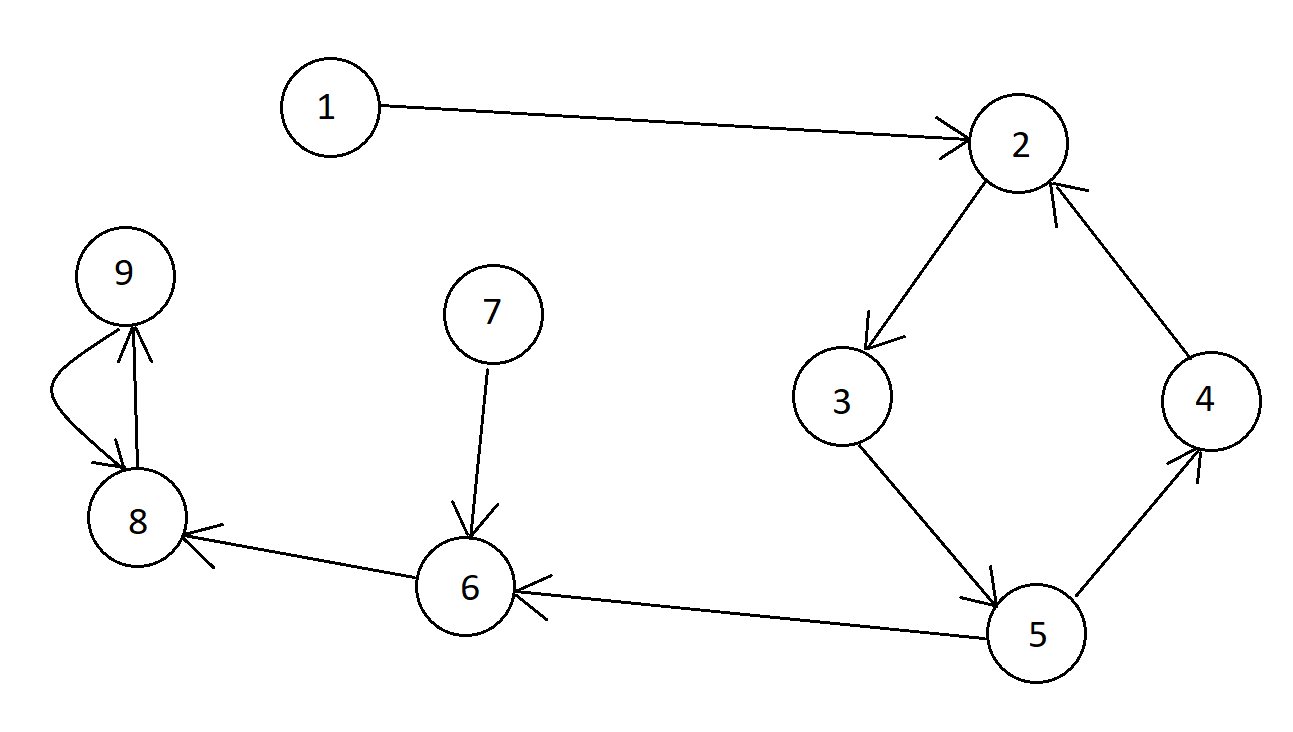
\includegraphics[width=6.2cm]{Conex.png}
    	\caption{Acest graf nu este tare conex pentru c\u a nu exist\u a drum de la 4 la 1, dar are 5 componente tare conexe: subgraful $\{2,3,4,5\}$, subgraful $\{8,9\}$ \c si 3 subgrafuri cu c\^ ate un singur nod:$\{1\}$,$\{6\}$ \c si $\{7\}$. }
    \end{figure}
    
    
    \chapter{Drumuri minime de surs\u a unic\u a}

    
    S\u a presupunem c\u a un ciclist dore\c ste s\u a parcurg\u a drumul de la Ia\c si la Bac\u au  utiliz\^and o hart\u a rutier\u a a Rom\^ aniei, unde sunt indicate distan\c tele \^ intre fiecare dou\u a intersec\c tii adiacente.
    
    O posibil\u a rezolvare a acestei probleme este aceea de a \^ in\c sirui toate drumurile de la Ia\c si la Bac\u au \c si, pe baza lungimilor acestora, de a alege cel mai scurt drum dintre ele. Este vizibil de observat faptul c\u a num\u arul de variante posibile este un num\u ar foarte mare chiar \c si \^ in cazul \^ in care avem drumuri care nu con\c tin cicluri.
    
    \^ In acest capitol vom ar\u ata cum poate fi rezolvat\u a problema \^ in mod eficient. \^ Intr-o \textbf{problem\u a de drum minim}, avem \^ in ipotez\u a un graf orientat ponderat $G=(V,E)$, iar func\c tia cost $f:E \longrightarrow \R $ repartizeaz\u a fiec\u arei muchii un cost exprimat printr-un num\u ar real. \textbf{Costul} drumului  $p=[ \alpha_{0},\alpha_{1},...,\alpha_{k}]$ reprezint\u a suma costurilor corespunz\u atoare muchiilor componente :
    \begin{equation*}
    f(p)=\sum\limits_{i=1}^{k} f(\alpha_{i-1},\alpha_{i})
    \end{equation*}
    
    A\c sadar, \textbf{costul unui drum minim} de la $u$ la $v$ este dat de
  	\begin{equation*}
  		\delta(u,v)=
  		\begin{cases}
  	    min\left\{f(p):u\leadsto v\right\},&\text{dac\u a exist\u a drum de la $u$ la $v$} \medskip\\
  		\infty,& \text{altfel} \medskip
  		\end{cases}
  		\end{equation*}
  		
  	\^ In cazul exemplului de mai sus, putem modela harta rutier\u a ca un graf: v\^arfurile constitue punctele de intersec\c tie, muchiile reprezint\u a segmentele de drum iar costurile, distan\c tele \^ intre intersec\c tii.
  	
  	\section{Reprezentarea drumurilor minime}
  	
  	Find dat un graf $G=(V,E)$, se va re\c tine pentru fiecare nod $v\in V$ un \textbf{predecesor} $\omega[v]$ care este fie un nod, fie NULL. Pentru determinarea drumurilor minime, algoritmii prezenta\c ti in acest capitol determin\u a $\omega$ a\c sa \^ inc\^ at pentru orice v\^ arf $v$, lan\c tul de predecesori care porne\c ste de la $v$ s\u a coincid\u a unei travers\u ari \^ in ordinea invers\u a a unui drum de valoare minim\u a de la v\^ arful surs\u a $s$ la $v$.
  	
  	Pe durata execu\c tiei a unui algoritm pentru determinarea  unui drum minim, valorile lui $\omega$ nu arat\u a \^ in mod necesar drumurile minime. Astfel, vom considera \textbf{subgraful predecesor} $G_{\omega}=(V_{\omega},E_{\omega})$, unde $V_{\omega}$ reprezint\u a mul\c timea v\^ arfurilor din $G$ cu proprietatea c\u a au predecesor diferit de NULL, reunit\u a cu mul\c timea constituit\u a din v\^arful $s$ :
  	
  	\vspace{0.2cm}	
  	$\centering V_{\omega}=\left\{v\in V :\omega[v]\ne NULL\right\}\cup \left\{s\right\}$
  	\vspace{0.1cm}
  		
  	Mul\c timea de muchii $E_{\omega}$ este mul\c timea de muchii impus\u a de valorile lui $\omega$ pentru v\^ arfurile din $V_{\omega}$ :
  	
  	\vspace{0.2cm}
  	$\centering E_{\omega}=\left\{(\omega [v],v)\in E : v\in V_{\omega}\setminus \left\{s\right\}\right\}$
  	\vspace{0.2cm}
  	
  	Valorile $\omega$ determinate de algoritmii ce vor fi prezenta\c ti, asigur\u a c\u a la terminare, $G_{\omega}$ s\u a fie un "arbore al drumurilor minime". Mai precis, exist\u a un arbore cu r\u ad\u acin\u a care con\c tine c\^ ate un drum minim de la sursa $s$ la orice nod al grafului care este accesibil din nodul surs\u a $s$. 
  	
  	Fie $G=(V,E)$ un graf orientat ponderat, av\^ and func\c tia de cost $f:E \longrightarrow \R$, presupunem c\u a graful $G$ nu con\c tine cicluri de cost negativ, disponible din v\^ arful surs\u a $s$, a\c sadar drumurile minime sunt bine definite. Un \textbf{arbore al drumurilor minime} de rad\u acin\u a $s$ este subgraful orientat $G'=(V',E')$ unde $V'\subseteq V$, $E'\subseteq E$ a.\^ i. urm\u atoarele condi\c tii sunt \^ indeplinite:
  	
  	\vspace{0.2cm}
  	1. $G'$ arbore  cu r\u ad\u acin\u a, av\^ and pe $s$ ca r\u ad\u acin\u a.
  	\vspace{0.1cm}
  	
  	2. $V'$ mul\c timea v\^ arfurilor accesibile din $s$ \^ in $G$.
  	\vspace{0.1cm}
  	
  	3. Pentru orice $v\in V'$ unicul drum de la $s$ la $v$ in $G'$ este un drum minim de la $s$ la $v$ \^ in $G$.
  	\vspace{0.1cm}
  	
  	Drumurile minime nu sunt \^ intotdeauna unice \c si \^ in consecin\c t\u a exist\u a mai mul\c ti arbori de drumuri minime.
  	 \begin{figure}[!hbt]
  		\centering
  		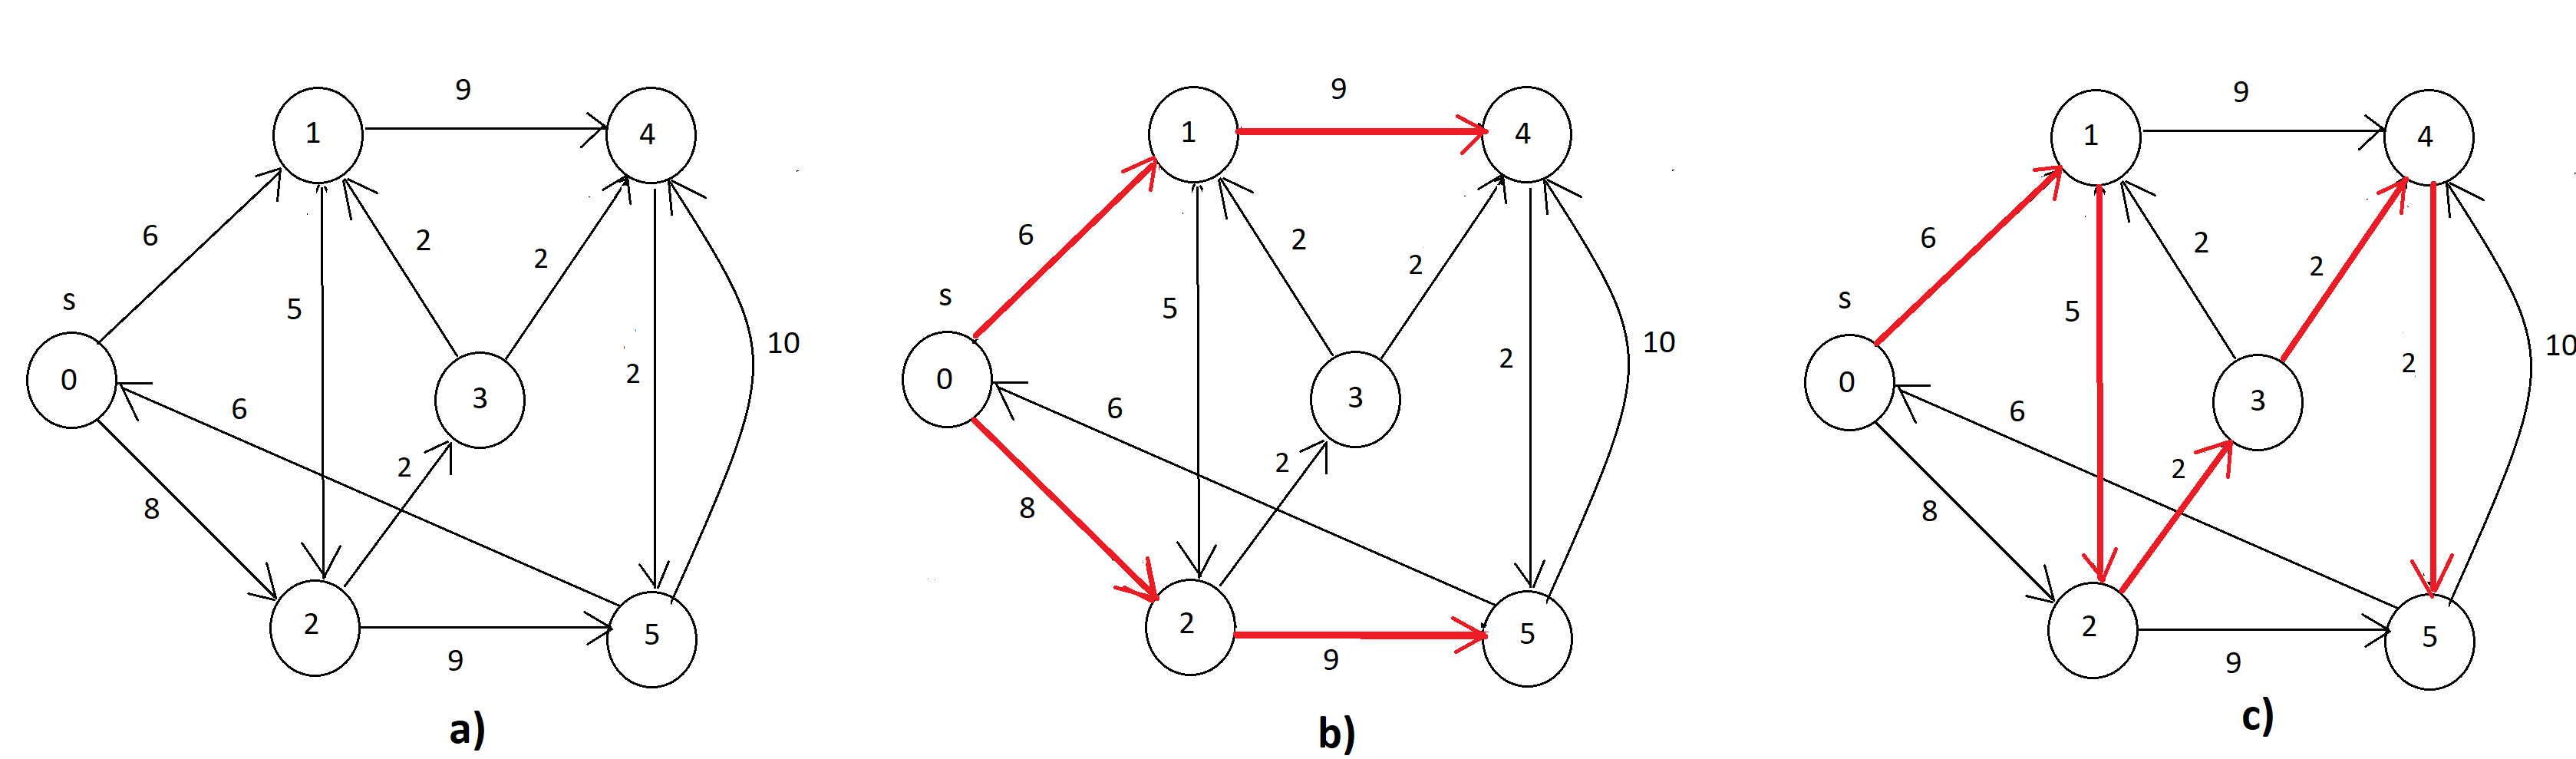
\includegraphics[width=12cm,height=4cm]{ArboreMinim.png}
  		\caption{ \textbf{a)} Graf orientat ponderat. \textbf{b)} Muchiile reprezentate cu ro\c su formeaz\u a un arbore de drumuri minime av\^ and ca r\u ad\u acin\u a sursa $s$. \textbf{c)} Un alt exemplu de arbore de drumuri minime av\^ and aceea\c si r\u ad\u acin\u a.}
  	\end{figure}
  	
  	\section{Relaxare}
  	
  	Algoritmii pentru determinarea drumurilor minime de surs\u a unic\u a sunt baza\c ti pe o tehnic\u a care poart\u a numele de \textbf{relaxare}. Pentru fiecare nod $v\in V$, conserv\u am un atribut $d[v]$, care reprezint\u a o margine superioar\u a a costului de drum minim de la $s$ la $v$. Numim acest atribut $d[v]$ o \textbf{estimare a drumului minim}. Estim\u arile predecesorilor \c si a drumurilor minime sunt ini\c tializate prin urm\u atorul algoritm:
  	
  	\vspace{0.2cm}
  	INI\c TIALIZEAZ\u A-SURS\u A-UNIC\u A ($G$,$s$)
  	
  	\vspace{0.1cm}
  	1: \textbf{for} fiecare v\^ arf $v\in V(G)$ 
  	
  	2: \hspace{0.5cm}$d[v]\longleftarrow \infty$

    3:\hspace{0.6cm}$\omega[v]\longleftarrow NULL$
    
    4: $d[s]\longleftarrow 0$
    
    Dup\u a ini\c tializare $\omega [v]=NULL$ pentru orice v\^ arf $v\in V$, $d[v] = 0$ pentru $v=s$ \c si $d[v] = \infty $ pentru $v\in V\setminus \{s\}$
    \begin{figure}[!hbt]
    \centering
    	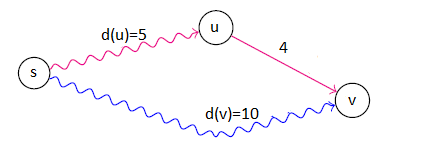
\includegraphics[width=10cm]{Relaxeaza.png}
    	\caption{Are loc procesul de relaxare a unei muchii $(u,v)$ cu costul $f(u,v)=4$. Pentru orice v\^ arf $u,v\in V$ este prezentat\u a estimarea drumului minim.  \^ Inainte de relaxare, $d[v] > d[u]+f(u,v)$, valoarea lui $d[v]$ descre\c ste \c si va fi egal\u a cu 9. \^ In cazul \^ in care $d[v]\leq d[u]+f(u,v)$, valoarea lui $d[v]$ va r\u am\^ ane neschimbat\u a.}
    \end{figure}

    Acest proces numit \textbf{relaxare} aplicat unei muchii $(u,v)$ verific\u a dac\u a drumul minim la $v$, poate fi \^ imbun\u at\u a\c tit pe baza lui $u$, \c si \^ in caz afirmativ se reactualizeaz\u a $d[v]$ \c si $\omega[v]$. Codul de mai jos realizeaz\u a un pas de relaxare a unei muchii $(u,v)$.
    
      	\vspace{0.3cm}
    RELAXEAZ\u A $(u,v,f)$
    
    \vspace{0.1cm}
    1: \textbf{if} $d[v] > d[u] + f(u,v)$ 
    
    2: \hspace{0.5cm}$d[v]\longleftarrow d[u] + f(u,v)$
    
    3:\hspace{0.6cm}$\omega[v]\longleftarrow u$
    
          	\vspace{0.3cm}
    \^ In figura 2.1 este aplicat algoritmul de mai sus, astfel estimarea drumului minim descre\c ste.
    
    To\c ti algoritmi apeleaz\u a INI\c TIALIZARE-SURS\u A UNIC\u A dup\u a care apeleaz\u a relaxarea repetat\u a a muchiilor. \^ In algoritmul Dijkstra fiecare muchie este relaxat\u a doar o singur\u a dat\u a iar \^ in cazul algoritmului Bellman-Ford, fiecare dintre muchii este relaxat\u a de mai multe ori.
    
    \section{Algoritmul Dijkstra}
    
    Algoritmul lui Dijkstra este cel mai utilizat algoritm de c\u autare pentru problema de drum minim. Algoritmul a fost propus de olandezul Edsger Dijkstra \^ in anul 1959. Algoritmul Dijkstra calculeaz\u a cel mai scurt drum  select\^ and v\^ arful nevizitat cu cea mai mic\u a distan\c t\u a fa\c t\u a de fiecare vecin nevizitat. Pentru un graf cu $n$ noduri av\^ and costuri negative pe muchii, metoda calculeaz\u a calea cu cel mai mic cost \^ intre o pereche de noduri cu o complexitate de $O(n^2)$. Algoritmul lui Dijkstra calculeaz\u a cel mai scurt drum de la nodul surs\u a p\^ an\u a la destina\c tie calcul\^ and iterativ cele mai scurte drumuri de la nodul surs\u a la toate celelalte noduri din graf.
    
    \subsection{Descrierea algoritmului}
    Fie un tablou $d[\,\,]$ unde pentru fiecare v\^ arf $v$ stoc\u am lungimea curent\u a a celui mai scurt drum de la $s$ la $v$ \^ in $d[v]$. Ini\c tial $d[s]=0$, iar pentru toate celelalte v\^ arfuri aceast\u a lungime este egal\u a cu INT$\_$MAX. \^ In implementare, un num\u ar suficient de mare (care este garantat a fi mai mare dec\^ at orice lungime posibil\u a) este ales ca infinit.
    \begin{equation*}
    d[v]=\infty,v\neq s
    \end{equation*}
    \^ In plus men\c tinem un tablou boolean $u[\,\,]$ care stocheaz\u a pentru fiecare v\^ arf $v$ dac\u a este marcat. Ini\c tial toate v\^ arfurile sunt nemarcate $u[v]=false$.
    
    
    Algoritmul lui Dijkstra ruleaz\u a pentru $n$ itera\c tii. Evident, \^ in  prima itera\c tie, v\^ arful de pornire $s$ va fi selectat. V\^ arful selectat $v$ este marcat. \^ In continuare, de la v\^ arful $v$ se realizeaz\u a relax\u ari: toate muchiile de forma $(v,i)$ sunt luate \^ in considerare \c si pentru fiecare v\^ arf $i$, algoritmul \^ incearc\u a s\u a \^ imbun\u at\u a\c teasc\u a valoarea $d[i]$. Dac\u a lungimea muchiei curente este egal\u a cu $f(v,i)$, atunci:
        \begin{equation*}
    d[i]=min(d[i],d[v]+f(v,i))
    \end{equation*}  
    Dup\u a ce toate aceste muchii sunt luate \^ in considerare, itera\c tia curent\u a se termin\u a. \^ In cele din urm\u a dup\u a $n$ itera\c tii, toate v\^ arfurile vor fi marcate \c si algoritmul se \^ incheie. Astfel, valorile g\u asite $d[v]$ sunt lungimile celor mai scurte drumuri de la $s$ la toate v\^ arfurile $v$.  
    O observa\c tie ar fi c\u a, dac\u a unele v\^ arfuri nu pot fi atinse din cele de \^ inceput, valorile $d[v]$ pentru ele vor r\u am\^ ane infinit. Evident, ultimele c\^ ateva itera\c tii ale algoritmului vor alege acele v\^ arfuri, dar nu se va lucra pentru ele. Prin urmare, algoritmul poate fi oprit imediat ce v\^ arful selectat are o distan\c t\u a infinit\u a fa\c t\u a de $s$. 
    
    \^ In esen\c t\u a, acest algoritm rezolv\u a eficient problema drumurilor minime de surs\u a unic\u a \^ intr-un graf orientat ponderat $G=(V,E)$, muchiile fiind nenegative. Vom presupune c\u a $f(u,v)\ge 0$ pentru fiecare $(u,v)\in E$.
    
    
    \vspace{0.3cm}
    DIJKSTRA $(G,f,s)$
    
    \vspace{0.1cm}
    1: INI\c TIALIZEAZ\u A-SURS\u A-UNIC\u A$(G,s)$
    
    2: $S\longleftarrow \emptyset$  
    
    3: $Q\longleftarrow V(G)$
    
    4: \textbf{while} $Q\ne \emptyset$ 
    
    5:\hspace{0.6cm} $u\longleftarrow$ EXTRAGE-MIN(Q)
    
    6:\hspace{0.6cm} $S\longleftarrow S\cup \{u\}$
    
    7:\hspace{0.6cm} \textbf{for} fiecare v\^ arf $v\in Adj[u]$\footnote{List\u a de adiacen\c t\u a care con\c tine toate nodurile $v$ pentru care exist\u a o muchie $(u,v)\in E$.} 
    
    8:\hspace{1.2cm} RELAXEAZ\u A$(u,v,f)$
    \vspace{0.3cm}
    
    
    Algoritmul Dijkstra aplic\u a metoda relaxare pentru fiecare muchie \^ in modul prezentat din figura 2.2.
    \begin{figure}[!hbt]
    	\centering
    	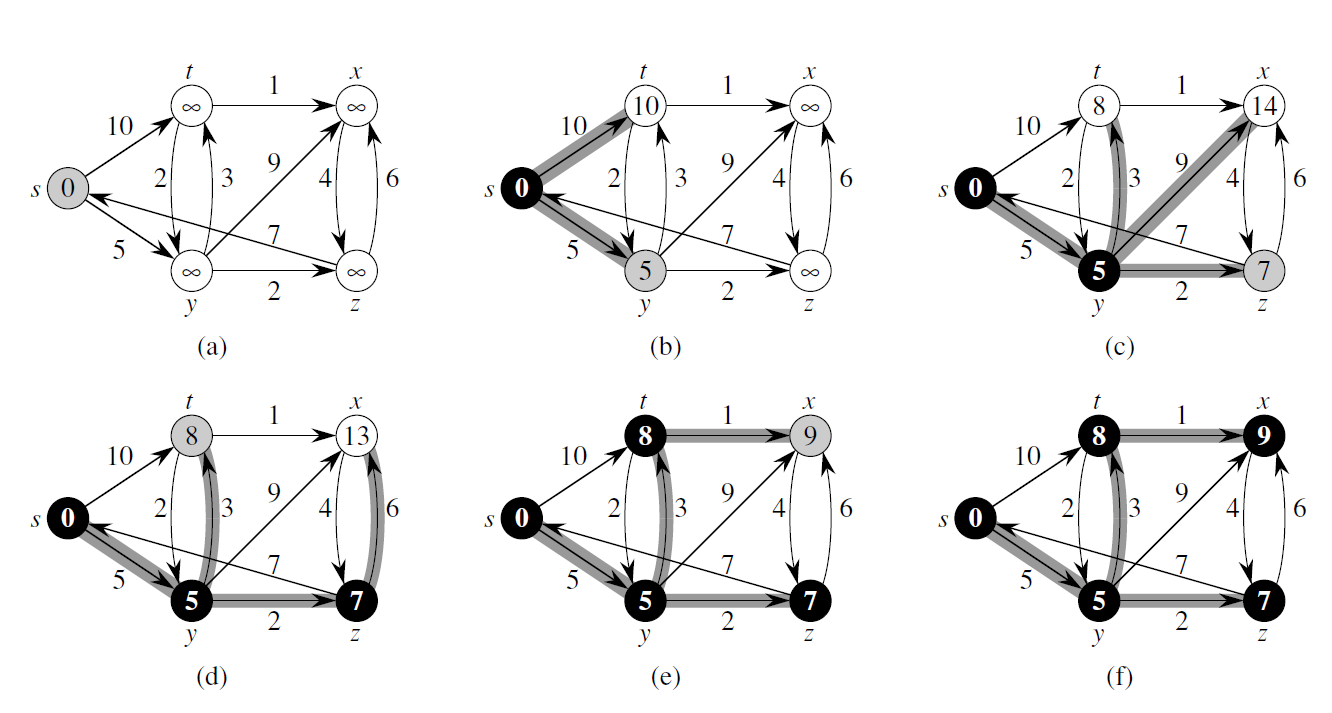
\includegraphics[width=13.2cm]{Dijkstra.png}
    	\caption{\cite{Cormen} Algoritmul Dijkstra pe etape. V\^ arful surs\u a este 0. Muchiile ha\c surate reprezint\u a valorile predecesorilor: dac\u a $(u,v)$ este ha\c surat atunci $\omega[v]=u$. V\^ arfurile marcate cu negru sunt din $S$ iar cele marcate cu alb apar\c tin cozii $Q=V-S$.\textbf{(a)} Configura\c tia exist\u a \^ inaintea primei itera\c tii a repeti\c tiei \textbf{while}. V\^ arful ha\c surat este $u$ din linia 5 \c si are valoarea minim\u a.\textbf{(b)-(f)} Configura\c tia dup\u a fiecare itera\c tie \textbf{while}.}
    \end{figure}

   \subsection{Implementare}
   
   
   Algoritmul Dijkstra efectueaz\u a $n$ itera\c tii. La fiecare itera\c tie, se selecteaz\u a un v\^ arf nemarcat $v$ cu cea mai mic\u a valoare $d[v]$, \^ il marcheaz\u a \c si verific\u a toate marginile $(v,i)$ \^ incerc\^ and s\u a \^ imbun\u at\u a\c teasc\u a valoarea $d[i]$. Fie un graf ponderat orientat sau neorientat cu $n$ noduri \c si $m$ muchii. 
   
   Durata de rulare a acestui algoritm const\u a \^ in :
   \begin{itemize}
   	\item $n$ c\u aut\u ari a unui nod cu cea mai mic\u a valoare $d[v]$ printe nodurile nemarcate.
   	\item $m$ \^ incerc\u ari de relax\u ari.
   \end{itemize}

Pentru cea mai simpl\u a implementare a acestor opera\c tii pe fiecare v\^ arf de itera\c tie, c\u autarea necesit\u a $O(n)$ opera\c tii \c si fiecare relaxare poate fi efectuat\u a \^ in $O(1)$. Prin urmare, comportamentul asimptotic rezultat al algoritmului este:
\begin{equation*}
O(n^2)\footnote{Alte rezultate cu privire la costul diverselor implemet\u ari a algoritmului lui Dijkstra, \cite{Sedgewick}}
\end{equation*}

Aceast\u a complexitate este optim\u a pentru un graf ponderat, atunci c\^ and $m\approx n^2$. Cu toate acestea, \^ in grafurile rare, c\^ and $m$ este mult mai mic dec\^ at num\u arul maxim de muchii $n^2$, problema poate fi rezolvat\u a \^ in complexitate $O(nlog(n)+m)$. 
    
     \begin{figure}[!hbt]
    	\centering
    	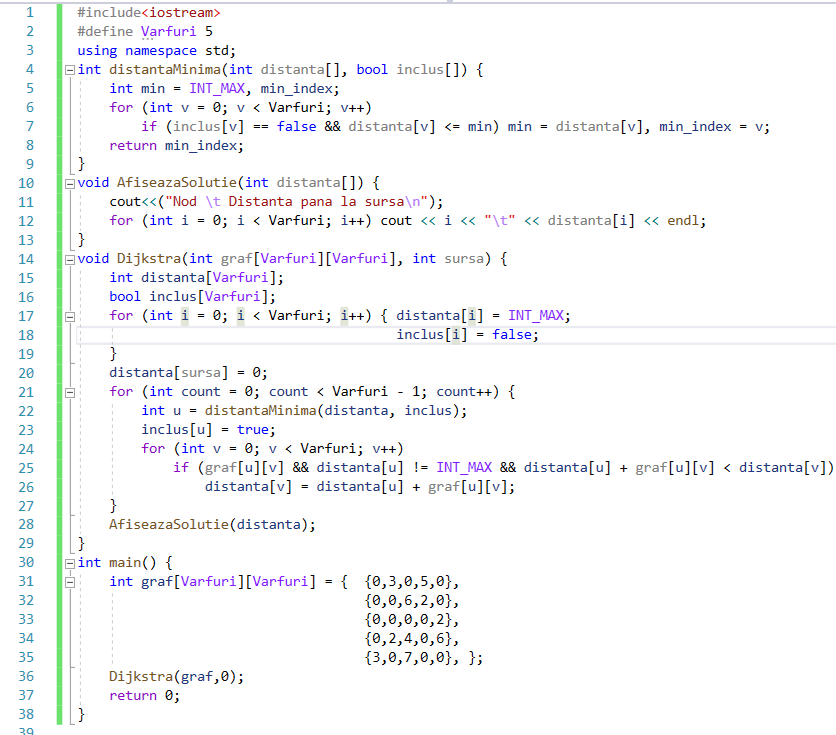
\includegraphics[width=12cm,height=9.1cm]{Dijkstra_cod1.png}
    	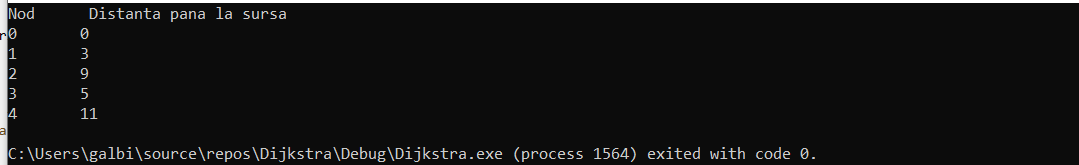
\includegraphics[width=12cm]{Dijkstra_output1.png}
    	\caption{Algoritmul afi\c seaz\u a toate costurile drumurilor de la $i$ la surs\u a.}
    \end{figure}
     \chapter{Drumuri minime \^ intre toate perechile de v\^ arfuri}
     
     \^ In acest capitol vom pune problema studiului determin\u arii drumurilor de lungime minim\u a \^ intre toate perechile de v\^ arfuri ale unui graf $G$. Problema poate fi dac\u a dorim s\u a construim un tabel al distan\c telor \^ intre toate perechile de magazine. Ipotezele sunt acelea\c si ca \^ in capitolul anterior, avem un graf orientat $G=(V,E)$, cu costuri \c si o func\c tie de costuri $f:E \longrightarrow \R $ aplicat\u a arcelor grafului. Dorim s\u a determin\u am, pentru fiecare $u,v\in V$, un \textbf{drum de cost minim} de la $u$ la $v$, unde acest rezultat este suma costurilor acelor arce care formeaz\u a acest drum. Rezultatul ob\c tinut este de preferat s\u a fie sub forma unui tabel: linia $u$, coloana $v$ \c si con\c tinutul drumului minim de la $u$ la $v$.
     
     Majoritatea algoritmilor din cadrul acestui capitol vor avea reprezentarea prin matrici de adiacen\c t\u a. Input-ul este o matrice $A$, av\^ and dimensiunea $n\times n$, reprezent\^ and costurile arcelor unui graf $G=(V,E)$ orientat cu $n$ noduri. Mai pe scurt $A=(a_{ij})$ unde
     \begin{equation*}
     a_{ij}=
    \begin{cases}
     0,&\text{dac\u a $i=j$}, \medskip\\
    f(i,j),& \text{dac\u a $i\ne j$ \c si $(i,j)\in E$}, \medskip\\
     \infty,&\text{dac\u a $i\ne j$ \c si $(i,j)\notin E$}.\medskip
    \end{cases}
     \end{equation*}
     Output-ul este o matrice $D=(d_{ij})$ de dimensiune $n\times n$ al c\u aror elemente reprezint\u a costul minim de la $i$ la $j$. Not\^ and cu $\delta(i,j)$  costul minim drumului de la $i$ la $j$, vom avea $d_{ij}=\delta(i,j)$.
     
     Pentru rezolvarea problemei, trebuie s\u a calcul\u am costurile drumurilor minime \c si \textbf{matricea predecesorilor} pe care o not\u am cu $P=(\pi_{ij})$, unde $\pi_{ij}$ este $NIL$ pentru $i=j$ sau dac\u a nu este un drum de la $i$ la $j$. Altfel, elementul $\pi_{ij}$ este predecesorul lui $j$ av\^ and un drum minim de la $i$. Pentru orice v\^arf $i\in V$, fix\u am \textbf{subgraful predecesorilor} lui $G$ pentru $i$ ca $G_{\pi,i}=(V_{\pi,i},E_{\pi,i})$, unde
     \begin{equation*}
     V_{\pi,i}=\{j\in V:\pi_{ij}\neq NIL\}\cup \{i\}
     \end{equation*}
     \c si 
     \begin{equation*}
     E_{\pi,i}=\{(\pi_{ij},j):j\in V_{\pi,i} \ \text{\c si} \ \pi_{ij}\neq NIL\}.
     \end{equation*}
     
     Dac\u a $G_{\pi,i} $ \^ indepline\c ste condi\c tia de a fi un arbore de drum minim, atunci are loc urm\u atoarea procedur\u a, aceea de a aplica metoda AFI\c SEAZ\u A-DRUM, care afi\c seaz\u a drumul minim de la $i$ la $j$.
     
       \vspace{0.3cm}
     AFI\c SEAZ\u A-DRUM $(P,i,j)$
     
     \vspace{0.1cm}
     1: \textbf{if} $i=j$ 
     
     2:\hspace{0.6cm} afi\c seaz\u a  $i$
     
     3: \textbf{else}
     
     4: \hspace{0.6cm}\textbf{if} $\pi_{ij}=NIL$ 
     
     5:\hspace{1.2cm} afi\c seaz\u a "Nu este drum de la $i$ la $j$" 
     
     6:\hspace{0.6cm} \textbf{else}
     
     7:\hspace{1.2cm} AFI\c SEAZ\u A-DRUM $(P,i,\pi_{ij})$
     
     8:\hspace{1.2cm} afi\c seaz\u a $j$
     \vspace{0.3cm}
     
     \section{Drumuri minime }
     
     Studiem mai \^ int\^ ai \textbf{structura unui drum minim} pentru caracterizarea unei solu\c tii optime. Presupunem  c\u a graful $G=(V,E)$ este reprezentat printr-o matrice de adiacen\c t\u a $A=(a_{ij})$. Consider\u am un drum $p$ de lungime minim\u a de la v\^ arful $i$ la $j$ \c si $m$ num\u arul de arce con\c tinute \^ in $p$. Dac\u a $i=j$ atunci costul lui $p$ este 0. Dac\u a $i\neq j$ atunci putem descompune drumul $p$ \^ in $i\xrightarrow{\text{p'}}k\rightarrow j$ unde $p'$ con\c tine $m-1$ arce. \^ In final avem urm\u atoarea egalitate 
     \begin{equation*}
     \delta (i,j)=\delta (i,k)+f(k,j).
     \end{equation*}
     
     Definim $d_{ij}^{(m)}$ ca fiind costul minim a unui drum de la $i$ la $j$ care este alc\u atuit din cel mult $m$ arce.
     \begin{equation*}
		d_{ij}^{(0)}=
		\begin{cases}
		0,&\text{dac\u a $i=j$}, \medskip\\
		\infty,&\text{dac\u a $i\ne j$}.\medskip
		\end{cases}
	 \end{equation*}
	 Pentru $m\geq 1$, determin\u am $d_{ij}^{(m)}$ ca minimul \^ intre $d_{ij}^{(m-1)}$ \c si costul minim al fiec\u arui drum de la $i$ la $j$ cu cel mult $m$ arce , lu\^ and \^ in considerare to\c ti predecesorii $k$ ai lui $j$.
	 \begin{equation}
	 d_{ij}^{(m)}=\text{min} \bigg( d_{ij}^{(m-1)},\min_{1\leq k \leq n} \bigg\{  d_{ik}^{(m-1)}+a_{kj}\bigg\} \bigg) = \min_{1\leq k \leq n}\bigg\{  d_{ik}^{(m-1)}+a_{kj}\bigg\}
	 \end{equation}
     iar costurile $\delta (i,j)$ ale drumurilor minime sunt date de 
          \begin{equation*}
     \delta (i,j)=d_{ij}^{(n-1)}=d_{ij}^{(n)}=d_{ij}^{(n+1)}=....
     \end{equation*}
     
     Dac\u a graful $G$ nu are nici un ciclu de cost negativ, putem deduce c\u a toate drumurile minime sunt elementare \c si con\c tin m\u acar, $n-1$ arce. Un drum de la nodul $i$ la  $j$ cu mai mult de $n-1$ arce nu poate avea un cost mai mic dec\^ at cel mai scurt drum de la nodul $i$ la $j$.
     
     Avem urm\u atoarea problem\u a, dorim s\u a determin\u am \^ in mod ascendent costurile drumurilor minime. Consider\u am ca input o matrice $A=(a_{ij})$ \c si vom determina o list\u a de matrici $D^{(1)},D^{(2)},...,D^{(n-1)}$, unde pentru orice $m=1,2,..,n-1$ avem $D^{(m)}=\big( d_{ij}^{(m)} \big)$. Matricea $D^{(n-1)}$ va con\c tine costurile drumurilor minime. O observa\c tie important\u a ar fi c\u a dac\u a $d_{i,j}^{(1)}=a_{ij}$ pentru orice $i,j\in V$, ob\c tinem $D^{(1)}=A$. Cu alte cuvinte, d\^ andu-se matricele $D^{(m-1)}$ \c si $A$, se va ob\c tine matricea $D^{(m)}$ care reprezint\u a extinderea drumurilor minime cu \^ inc\u a un arc.
     
     \vspace{0.3cm}
     EXTINDE$(D,A)$
     
     \vspace{0.1cm}
     1: $n\leftarrow linii[D]$
     
     2: fie $B=(b_{ij})$ matrice cu dimensiunea $n\times n$ 
     
     3: \textbf{for} $i\leftarrow 1,n$ 
     
     4: \hspace{0.6cm}\textbf{for} $j\leftarrow 1,n$ 
     
     5:\hspace{1.2cm} $b_{ij}\leftarrow \infty$
     
     6:\hspace{1.2cm} \textbf{for} $k\leftarrow 1,n$ 
     
     7:\hspace{1.8cm} $b_{ij}\leftarrow $min$(b_{ij},d_{ik}+a_{kj})$
     
     8: \textbf{return} B
     \vspace{0.3cm}
     
     Timpul de execu\c tie al acestei func\c tii este de $O(n^3)$ datorit\u a celor 3 bucle pe care le con\c tine. Func\c tia returneaz\u a matricea $B=(b_{ij})$, acest lucru realiz\^ anduse cu ajutorul ecu\c tiei (3.1) pentru orice $i,j$ utiliz\^ and $D$ pentru $D^{(m-1)}$ \c si $B$ pentru $D^{(m)}$.
     
     Acum, dup\u a toat\u a aceast\u a discu\c tie, putem observa leg\u atura cu \^ inmul\c tirea matricilor. Dorim s\u a calcul\u am produsul dintre  dou\u a matrici $A$ \c si $B$ de dimensiune $n\times n$, $C=A*B$. Vom calcula pentru orice $i,j=1,2,....,n$
     \begin{equation}\footnote{Se poate ar\u ata c\u a pornind de la (3.2) se ajunge la (3.1). \cite{Cormen}}
     c_{ij}=\sum_{k=1}^{n} a_{ik}*b_{kj}.
     \end{equation}
     
          \vspace{0.3cm}
     \^ INMUL\c TE\c STE-MATRICILE$(A,B)$
     
     \vspace{0.1cm}
     1: $n\leftarrow linii[A]$
     
     2: fie $C=(c_{ij})$ matrice cu dimensiunea $n\times n$ 
     
     3: \textbf{for} $i\leftarrow 1,n$ 
     
     4: \hspace{0.6cm}\textbf{for} $j\leftarrow 1,n$ 
     
     5:\hspace{1.2cm} $c_{ij}\leftarrow 0$
     
     6:\hspace{1.2cm} \textbf{for} $k\leftarrow 1,n$ 
     
     7:\hspace{1.8cm} $c_{ij}\leftarrow c_{ij}+a_{ik}*b_{kj}$
     
     8: \textbf{return } C
     \vspace{0.3cm}
     
     \^ Intorc\^ andu-ne la problema propriu zis\u a, determin\u am costul drumurilor minime  extinz\^ and arc cu arc. Not\^ and cu $A*B$ matricea returnat\u a de EXTINDE(A,B), determin\u am \c sirul de $n-1$ matrice
	\begin{gather*}
         D^{(1)}=D^{(0)}*A=A,\medskip\\
   		 D^{(2)}=D^{(1)}*A=A^{2},\\
   		 \vdots \\
   		 D^{(n-1)}=D^{(n-2)}*A=A^{n-1}.
	\end{gather*}
	
	Acum c\u a am determinat \c sirul de $n-1$ matrice, putem transpune tot ce am scris mai sus \^ intr-o func\c tie.
	
	          \vspace{0.3cm}
	DRUMURI-MINIME$(A)$
	
	\vspace{0.1cm}
	1: $n\leftarrow linii[A]$
	
	2: $D^{(1)}\leftarrow A $
	
	3: \textbf{for} $i\leftarrow 2,n-1$ 
	
	4: \hspace{0.6cm} $D^{(i)}\leftarrow $EXTINDE ($D^{(i-1)},A$)
	
	5: \textbf{return} $D^{(n-1)}$
	\vspace{0.3cm}
    
    Acest\u a func\c tie este o versiune mai lent\u a, timpul de execu\c tie al determin\u arii acestui \c sir fiind de $O(n^4)$.
    
    \section{Algoritmul Floyd-Warshall}
    
    \^ In informatic\u a, algoritmul Floyd-Warshall (cunoscut \c si sub numele de algoritmul lui Floyd, algoritmul Roy-Warshall, algoritmul Roy-Floyd) este un algoritm pentru g\u asirea drumurilor celor mai scurte \^ intr-un graf ponderat cu cost pozitiv sau negativ. O singur\u a execu\c tie a algoritmului va g\u asi lungimile ale celor mai scurte drumuri \^ intre toate perechile de v\^ arfuri. De\c si acest algoritm nu \^ intoarce detalii ale drumurilor \^ in sine, este posibil\u a reconstruc\c tia drumurilor cu modific\u ari simple ale algoritmului.
    
    \subsection{Descrierea algoritmului}
    
    Ideea principal\u a a acestui algoritm este de a parti\c tiona procesul de g\u asire a celui mai scurt drum \^ intre oricare dou\u a noduri, la mai multe faze. Astfel, algoritmul ia \^ in considerare nodurile "intermediare" ale unui drum minim, unde un \textit{nod intermediar} al unui drum elementar $p=[v_1,v_2,...,v_n]$ este orice nod din mul\c timea $\{v_2,v_3,...,v_{n-1}\}$.
    
    Fie $V=\{1,2,...,n\}$ mul\c timea nodurilor lui $G$ \c si matricea $D=(d_{ij})$ ale c\u aror elemente reprezint\u a distan\c ta de la $i$ la $j$, pentru orice $i,j=\overline{1,2,...,n}$. \^ Inainte de pasul $k$ ($k=1,...,n$), $d[i][j]$ stocheaz\u a lungimea celui mai scurt drum de la nodul $i$ la $j$ care con\c tine doar v\^ arfurile $\{1,2,...,k\}$ ca v\^ arfuri interne. Pentru orice pereche $(i,j)\in V\times V$, consider\u am toate drumurile de la $i$ la $j$ ale c\u aror noduri intermediare fac parte din mul\c timea $\{1,2,...,k\}$. Fie $p$ drumul de cost minim dintre aceste drumuri.
    
    Este u\c sor de ar\u atat c\u a proprietatea are loc pentru primul pas. Pentru $k=0$, putem \^ inc\u arca matricea cu $d[i][j]=f(i,j)$ dac\u a exist\u a muchie de la $i$ la $j$ cu costul $f(i,j)$ \c si $d[i][j]=\infty$ dac\u a nu exist\u a nici o muchie. \^ In principiu, \^ in aplica\c tii, aproxim\u am $\infty$ cu un num\u ar foarte mare.
    
    S\u a presupunem c\u a ne afl\u am la pasul $k$, \c si vrem s\u a construim matricea $d[\ ][\ ]$ astfel \^ inc\^ at s\u a \^ indeplineasc\u a cerin\c tele pentru pasul $(k+1)$. Trebuie s\u a remediem distan\c tele pentru unele perechi de noduri $(i,j)$. \cite{Cormen} Exist\u a dou\u a cazuri fundamentale care depind de statutul lui $k$:
     \begin{itemize}
    	\item Dac\u a nodul $k$ nu este nod intermediar al drumului $p$, atunci cel mai scurt drum de la nodul $i$ la $j$ cu nodurile interne $\{1,2,...,k\}$ coincide cu cel mai scurt drum cu nodurile interne din  $\{1,2,...,k-1\}$. \^ In acest caz, $d[i][j]$ va r\u am\^ ane neschimbat \^ in timpul tranzi\c tiei.
    	\item Dac\u a nodul $k$ este nod intermediar al drumului $p$, atunci drumul poate fi descompus \^ in dou\u a drumuri, fiecare folosind nodurile din $\{1,2,...,k-1\}$ pentru a compune un drum care folose\c ste toate nodurile din $\{1,2,...,k\}$. Asta \^ inseamn\u a c\u a putem \^ imp\u ar\c ti drumul de la $i$ la $j$ \^ in dou\u a drumuri: un drum de la $i$ la $k$ iar cel de-al doilea de la $k$ la $j$. Prin urmare am calculat deja lungimile acestor drumuri \^ inainte \c si putem calcula lungimea celui mai scurt drum de la $i$ la $j$ ca fiind $d[i][k]+d[k][j]$.
    \end{itemize}
\vspace{0.5cm}	
\hspace{1.6cm} {\scriptsize	toate nodurile intermediare \hspace{0.5cm} toate nodurile intermediare 
	
	\hspace{1.6cm}	din  $\{1,2,...,k-1\}$  \hspace{1.7cm}	din  $\{1,2,...,k-1\}$}
\begin{figure}[!hbt]
	\centering
	\hspace{0.5cm}
	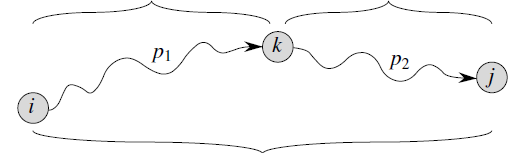
\includegraphics[width=7.2cm,height=2cm]{Warshall.png}
	\newline
	{\scriptsize $p$: toate nodurile intermediare din $\{1,2,...,k\}$}
	\caption{Drumul p este unul de lungime minim\u a de la nodul $i$ la $j$ iar $k$ este nodul intermediar al lui $p$ cu num\u arul cel mai mare. Drumul $p_1$ reprezint\u a por\c tiunea din drumul $p$ de la $i$ la $k$ cu toate nodurile intermediare $\{1,2,...,k-1\}$. Aceea\c si procedur\u a este valabil\u a \c si pentru drumul $p_2$.}
\end{figure}


	Combin\^and aceste dou\u a cazuri, afl\u am c\u a putem recalcula lungimea tuturor perechilor $(i,j)$ la pasul $k$ \^ in felul urm\u ator:
	 \begin{equation*}
	d_{nou}[i][j]=min(d[i][j],d[i][k]+d[k][j])
	\end{equation*}	
	Astfel, tot ce este necesar la pasul $k$ este de a itera peste toate perechile de v\^ arfuri \c si de a recalcula lungimea celui mai scurt drum dintre ele. Prin urmare, dup\u a pasul $n$, valoarea $d[i][j]$ din matricea cost $D$ este lungimea celui mai scurt drum dintre $i$ \c si $j$ sau $\infty$ dac\u a  nu exist\u a drum de la $i$ la $j$.


	O ultim\u a remarc\u a ar fi c\u a nu ar trebui s\u a cre\u am o alta matrice $D_{nou}$ pentru stocarea temporal\u a a celui mai scurt drum la pasul $k$, toate modific\u arile pot avea loc \^ in matricea $D$ la orice pas.
     \subsection{Implementare}
     
     Fie $D\in M_{n\times n}$ matricea cost care este construit\u a la pasul $k=0$ cum am men\c tionat mai sus. Deasemenea vom fixa elementele de pe diagonala principal\u a $d[i][i]=0$ pentru orice $i\in V$ la pasul 0.
     
     Algoritmul este implementat astfel:
     \begin{figure}[!hbt]
     	\centering
     	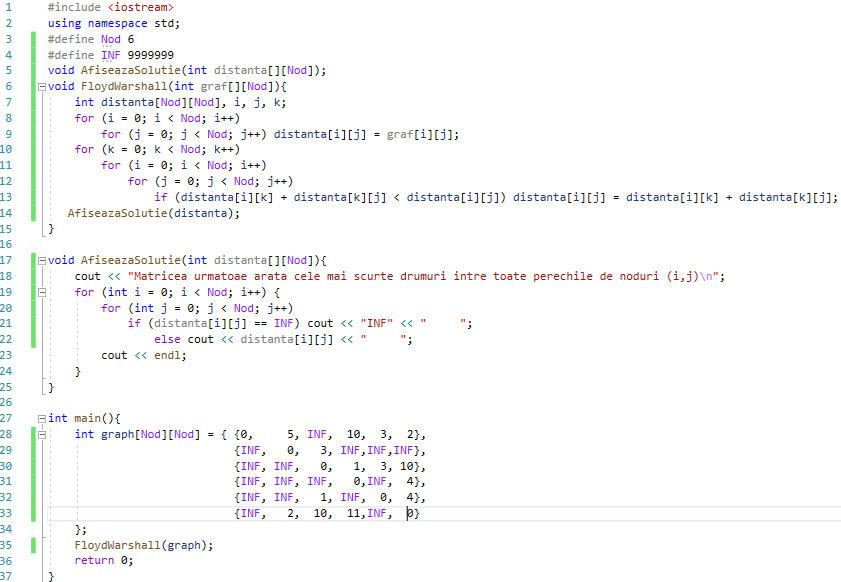
\includegraphics[width=12cm]{RoyFloysAlg.png}

     	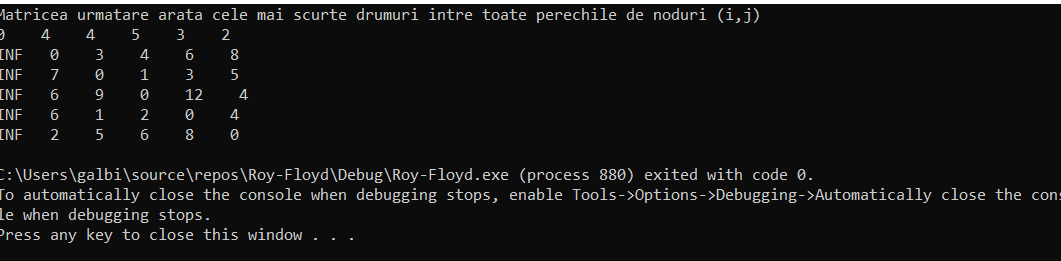
\includegraphics[width=12cm,height=2cm]{RFoutput.png}
     	\caption{Algoritmul afi\c seaz\u a toate drumurile de cost minim de la nodul $i$ la $j$ \^ in $k$ pa\c si.}
     \end{figure}
 
 	\chapter{Flux maxim} 
 
 
 	Problema fluxului maxim, la fel ca alte probleme formulate pe grafuri, \^ i\c si are originea \^ in economia modern\u a, mai precis \^ in optimizarea economic\u a. Cele mai recente aplica\c tii sunt \^ in domeniul re\c telelor \c si fluxurilor informa\c tionale. Dac\u a este pus\u a problema cercet\u arii unei re\c tele de transport a unui material dintr-un punct din care acesta este fabricat, acest punct \^ il numim surs\u a, \^ intr-un punct de depozitare pe care \^ il numin stoc sau destina\c tie folosind canale de transport cu anumite capacit\u a\c ti, iminent se ive\c ste  problema determin\u arii capacit\u a\c tii de transportare a materialului din surs\u a c\u atre stoc raport\^ andu-se la toat\u a re\c teaua. Cu alte cuvinte problema fluxului este aceea de a determina cantitatea cea mai mare de material care poate fi transportat\u a pornind de la surs\u a \c si ajung\^ and la destina\c tie \c tin\^ and cont de restric\c tiile de capacitate. Canalele de transport \c si materialele pot avea diverse forme precum: pachete de date, piese \c si transportatoare, conducte, cisterne petroliere, etc.
 	
 	\^ In ceea ce urmeaz\u a vom defini cu ajutorul grafurilor, re\c telele de transport, vom discuta anumite propriet\u a\c ti, vom defini problema fluxului maxim \c si vom introduce c\^ ateva nota\c tii utile.
 	\section{Fluxuri \c si re\c tele de transport}
 	
 	O \textbf{re\c tea de transport} este \^ in principiu un graf orientat $G=(V,E)$ \^ in care fiec\u arei muchii $(u,v)\in E$ cu $u,v \in V$ \^ ii este ata\c sat\u a o \textbf{capacitate} nenegativ\u a $c(u,v)\geq 0$. Vom denumi dou\u a v\^ arfuri din re\c tea: unul \textbf{surs\u a} $s$ \c si cel\u alalt \textbf{destina\c tie} $d$. Dac\u a  $(u,v)\notin E$ atunci consider\u am c\u a $c(u,v)=0$. Presupunem c\u a pentru orice nod $v\in V$ exist\u a un drum $s\rightarrow v\rightarrow d$. Graful fiind conex avem urm\u atoarea rela\c tie $|E|\geq |V|-1$.
 	
 	Fie o re\c tea de transport $G=(V,E)$ cu o func\c tie de capacitate $c$. Fix\u am nodul surs\u a $s$ \c si nodul destina\c tie $d$. Denumim \textbf{fluxul} $G$ ca fiind o func\c tie $f:V\times V\rightarrow \R$ care satisface urm\u atoarele condi\c tii:
 	\begin{enumerate}
 		\item \textbf{Restric\c tia de capacitate:} Pentru orice $u,v\in V$, $f(u,v)\leq c(u,v)$.
 		\item \textbf{Antisimetrie:} Pentru orice   $u,v\in V$, $f(u,v)=-f(v,u)$.
 		\item \textbf{Conservarea fluxului:} Pentru orice $u\in V\setminus \{s,d\}$ avem
 		\begin{equation*}
 	\sum\limits_{v\in V} f(u,v)=0.
 		\end{equation*}
 	\end{enumerate}
 	
 	
 	Cantitatea $f(u,v)$ care poate fi negativ\u a sau pozitiv\u a se nume\c ste \textbf{fluxul} pe arcul $(u,v)$. Totu\c si un flux negativ de la $u$ la $v$ reprezint\u a unul virtual, acesta nu reprezint\u a un transport profitabil, ci doar sugereaz\u a c\u a exist\u a un transport fizic de la $u$ la $v$. Definim valoarea fluxului ca fiind :
 	 		\begin{equation*}
 	|f|=\sum\limits_{v\in V} f(s,v),
 	\end{equation*}
 	mai precis fluxul total care pleac\u a din surs\u a. O prima observa\c tie ar fi c\u a nota\c tia pe care am definit-o mai sus  $|\cdot|$ nu \^ inseamn\u a valoarea absolut\u a sau cardinalul unei mul\c timi, ci  \textbf{valoarea fluxului}.
 	
 \begin{figure}[!hbt]
 	\centering
 	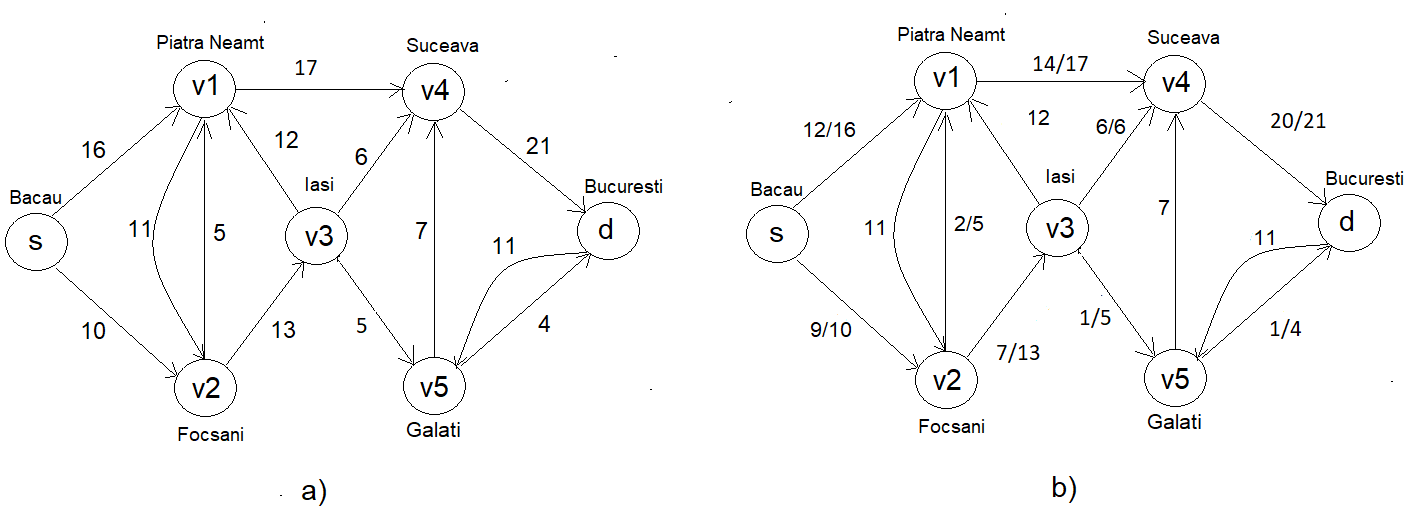
\includegraphics[width=12cm,height=5cm]{Flux.png}
 	\caption{\textbf{a)} O re\c tea $G$ pentru problema de transport de persoane a firmei BRONSON. Plecarea microbuzului din ora\c sul Bac\u au reprezint\u a sursa $s$ iar destina\c tia este dat\u a de nodul $d$. Persoanele sunt transportate prin localit\u a\c ti intermediare, dar numai $c(u,v)$ persoane pot fi luate din ora\c sul $u$ \^ in ora\c sul $v$. Toate arcurile au o anumit\u a capacitate. \textbf{b)} Valoarea fluxului $|f|=21$. Pe arce sunt marcate numai fluxurile de re\c tea pozitiv\u a. Dac\u a $f(u,v)>0$ rezult\u a c\u a arcul $(u,v)$ se poate marca astfel $f(u,v)/c(u,v)$ (scrierea pe care am folosit-o este doar de nota\c tie, aceea de a separa cele dou\u a valori: fluxul \c si capacitatea). Dac\u a $f(u,v)\leq 0$ atunci $(u,v)$ este marcat numai cu capacitatea. }
 \end{figure}

O prim\u a observa\c tie ar fi c\u a fluxul \^ intre oricare dou\u a v\^ arfuri care nu sunt legate prin nici un arc nu poate fi dec\^at 0. Astfel, pentru $(u,v)\notin E$ \c si $(v,u)\notin E$ avem $c(u,v)=c(v,u)=0$. Impun\^ andu-se restric\c tia de capacitate avem c\u a $f(u,v)\leq 0$ \c si $f(v,u)\leq 0$. Folosind antisimetria  $f(u,v)=-f(v,u)$ rezult\u a c\u a $f(u,v)=f(v,u)=0$. Prin urmare, existen\c ta fluxului nenul \^ intre $u$ \c si $v$ implic\u a $(v,u)\in E$ sau $(u,v)\in E$ sau ambele. 

	Acum apare urm\u atoarea problem\u a. Fiind dat $G$ o re\c tea de transport cu sursa $s$ \c si destina\c tia $d$, problema ne cere s\u a afl\u am  g\u asirea unui flux de valoare maxim\u a de la $s$ la $d$. Cu alte cuvinte, \textbf{problema fluxului maxim} impune g\u asirea unui flux maxim de la $s$ la $d$.
 
 	\section{Metoda lui Ford-Fulkerson}
 	
 	
   	Este denumit\u a "metod\u a" deoarece cuprinde mai multe implement\u ari, fiecare dintre acestea av\^ and timpul ei de execu\c tie. Metoda lui Ford-Fulkerson se bazeaz\u a pe trei idei principale: \textbf{re\c tele reziduale}, \textbf{drumuri de ameliorare} \c si\textbf{ t\u aieturi}.
   	
   	Metoda lui Ford-Fulkerson este una iterativ\u a. Pentru orice $u,v\in V$ vom avea fluxul $f(u,v)=0$. La fiecare itera\c tie vom m\u ari  fluxul prin g\u asirea unui "drum de ameliorare". Se va repeta acest procedeu p\^ ana nu se va mai g\u asi nici un drum de ameliorare.

   	
   	
   	  Fie $G=(V,E)$ o re\c tea de transport av\^ and o surs\u a $s$ \c si destina\c tia $d$. Consider\u am un flux $f$ \^ in $G$ \c si o pereche de v\^ arfuri $u,v\in V$. Denumim \textbf{capacitatea rezidual\u a} a arcului $(u,v)$ ca fiind cantitatea de flux adi\c tional\u a care poate fi transportat\u a de la $u$ la $v$, f\u ar\u a a dep\u a\c si capacitatea $c(u,v)$.
   	   		\begin{equation*}
   	  c_{f}(u,v)=c(u,v)-f(u,v)
   	  \end{equation*}
   	  
   	   \begin{figure}[!hbt]
   	  	\centering
   	  	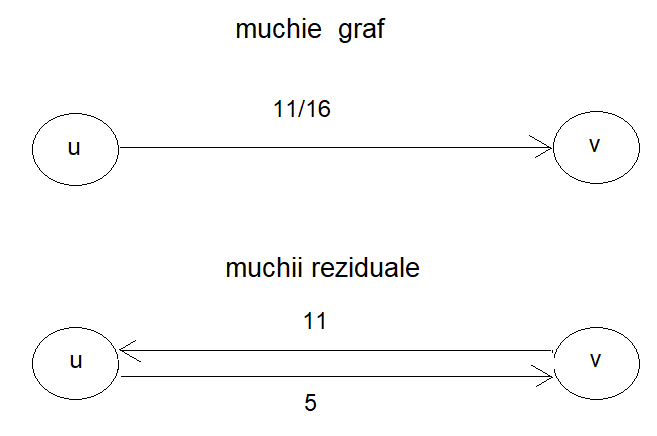
\includegraphics[width=7cm]{MuchiiReziduale.png}
   	  \end{figure}
   	  
   	  
   	  Dac\u a avem  arcul $(u,v)\in V$ cu $f(u,v)=11$ \c si $c(u,v)=16$ atunci se pot transporta $c_f(u,v)=5$ unit\u a\c ti suplimentare. De\c si arcul $(v,u)\notin V$, aplic\^ and antisimetria, vom putea avea totu\c si o capacitate rezidual\u a $c_f(v,u)=c(v,u)-f(v,u)=0-(-11)=11$. Astfel putem transporta 11 unit\u a\c ti \^ in sens opus care s\u a le anuleze pe cele 11 ale fluxului $f(u,v)$.
   	  
   	  
   	  Fiind dat $G$ \c si un flux $f$, numin \textbf{re\c teaua rezidual\u a} a lui $G$ de $f$ ca fiind $G_f=(V,E_f)$, unde 
     \begin{equation*}
	  E_f=\{(u,v)\in V\times V|\ c_f(u,v)=c(u,v)-f(u,v) >0 \}
	  \end{equation*} 	
   	


   	
  Denumim \textbf{drum de ameliorare} $p$ ca fiind un drum simplu de la $s$ la $t$ \^ in $G_f$. Mai general, drumul de ameliorare este un drum $[u_1,u_2,...,u_k]$, unde $u_1=s$ \c si $u_k=t$, \^ in graful rezidual cu $c_f(u_i,u_{i+1})>0$ pentru orice $i=1,2,...,k-1$. Spunem c\u a \textbf{capacitatea rezidual\u a} a lui $p$ reprezint\u a cantitatea maxim\u a a fluxului $f$ care poate fi transportat\u a de-a lungul drumului $p$, cu urm\u atoarea formul\u a
       \begin{equation*}
 c_f(p)=min\{c_f(u,v)|(u,v)\in p\}
  \end{equation*}
  \subsection{Implementare}
   La fiecare itera\c tie c\u aut\u am un drum aleator de amelioare $p$ la care m\u arim fluxul $f$ de-a lungul lui $p$ cu capacitatea rezidual\u a $c_f(p)$. Metoda urm\u atoare calculeaz\u a fluxul maxim a grafului $G=(V,E)$, actualiz\^ and fluxul $f(u,v)$. Dac\u a $u$ \c si $v$ nu formeaz\u a un arc atunci vom presupune c\u a $f(u,v)=0$. Presupunem c\u a \^ intre v\^ arfurile $u$ \c si $v$ valoarea capacit\u a\c tii este dat\u a de func\c tia $c(u,v)$, calculabil\u a \^ in timp constant \c si c\u a $c(u,v)=0$ dac\u a $(u,v)\notin E$.
   	
   	\vspace{0.3cm}
   	METODA-FORD-FULKERSON$(s,d,G)$  	
   	\vspace{0.1cm}
   	
   	1: \textbf{for} fiecare arc $(u,v)\in E[G]$ 
   	
   	2: \hspace{0.6cm} $f(u,v)\leftarrow 0$
   	
   	3: \hspace{0.6cm} $f(v,u)\leftarrow 0$
   	
   	4: \textbf{while} exist\u a un drum de la $s$ la $d$  \^ in re\c teaua rezidual\u a $G_f$ 
   	
   	5: \hspace{0.6cm} $c_f(p)\leftarrow min\{c_f(u,v)|(u,v)\in p\}$
   	
   	6: \hspace{0.6cm} \textbf{for} fiecare $(u,v)$ din $p$ 
   	
   	7:\hspace{1.2cm} $f(u,v)\leftarrow f(u,v)+c_f(p)$
   	
   	8:\hspace{1.2cm} $f(u,v)\leftarrow -f(u,v)$
   	\vspace{0.3cm}
   	
   	
   	Timpul de execu\c tie al acestui algoritm depinde de felul cum se calculeaz\u a drumul de ameliorare $p$ pe linia 4 a algoritmului. De cele mai multe ori, problemele de flux maxim apar cu capacit\u a\c ti care sunt numere \^ intregi.  \^ In cazul \^ in care capacit\u a\c tile sunt numere ra\c tionale, le putem \^ inlocui cu numere \^ intregi f\u ac\^ and o opera\c tie de scalare corespunz\u atoare.
   	
   	O implementare direct\u a al accestui algoritm dureaz\u a $O(E|f_m|)$, unde $f_m$ este fluxul maxim g\u asit de algoritm. Motivul pentru acest rezultat ar fi c\u a bucla \textbf{while} se execut\u a de cel mult $|f_m|$ ori deoarece valoarea fluxului cre\c ste cu cel pu\c tin o unitate de fiecare dat\u a. 
   	
   	Complexitatea algoritmului poate fi \^ imbun\u at\u a\c tit\u a dac\u a $p$ de pe linia 4 se calculeaz\u a folosind o c\u autare \^ in l\u a\c time, care acest lucru garanteaz\u a c\u a va fi calea \textit{cea mai scurt\u a} de la $s$ la $t$ \^ in re\c teaua rezidual\u a, unde  fiecarei muchii \^ ii corespunde o distan\c t\u a unitar\u a (greutate). Vom numi aceast\u a implementare a metodei ca fiind \textbf{algoritmul lui Edmons-Karp}.
   	
   	
   	
   \vspace{0.3 cm}\begin{figure}[!hbt]
  	\centering
  	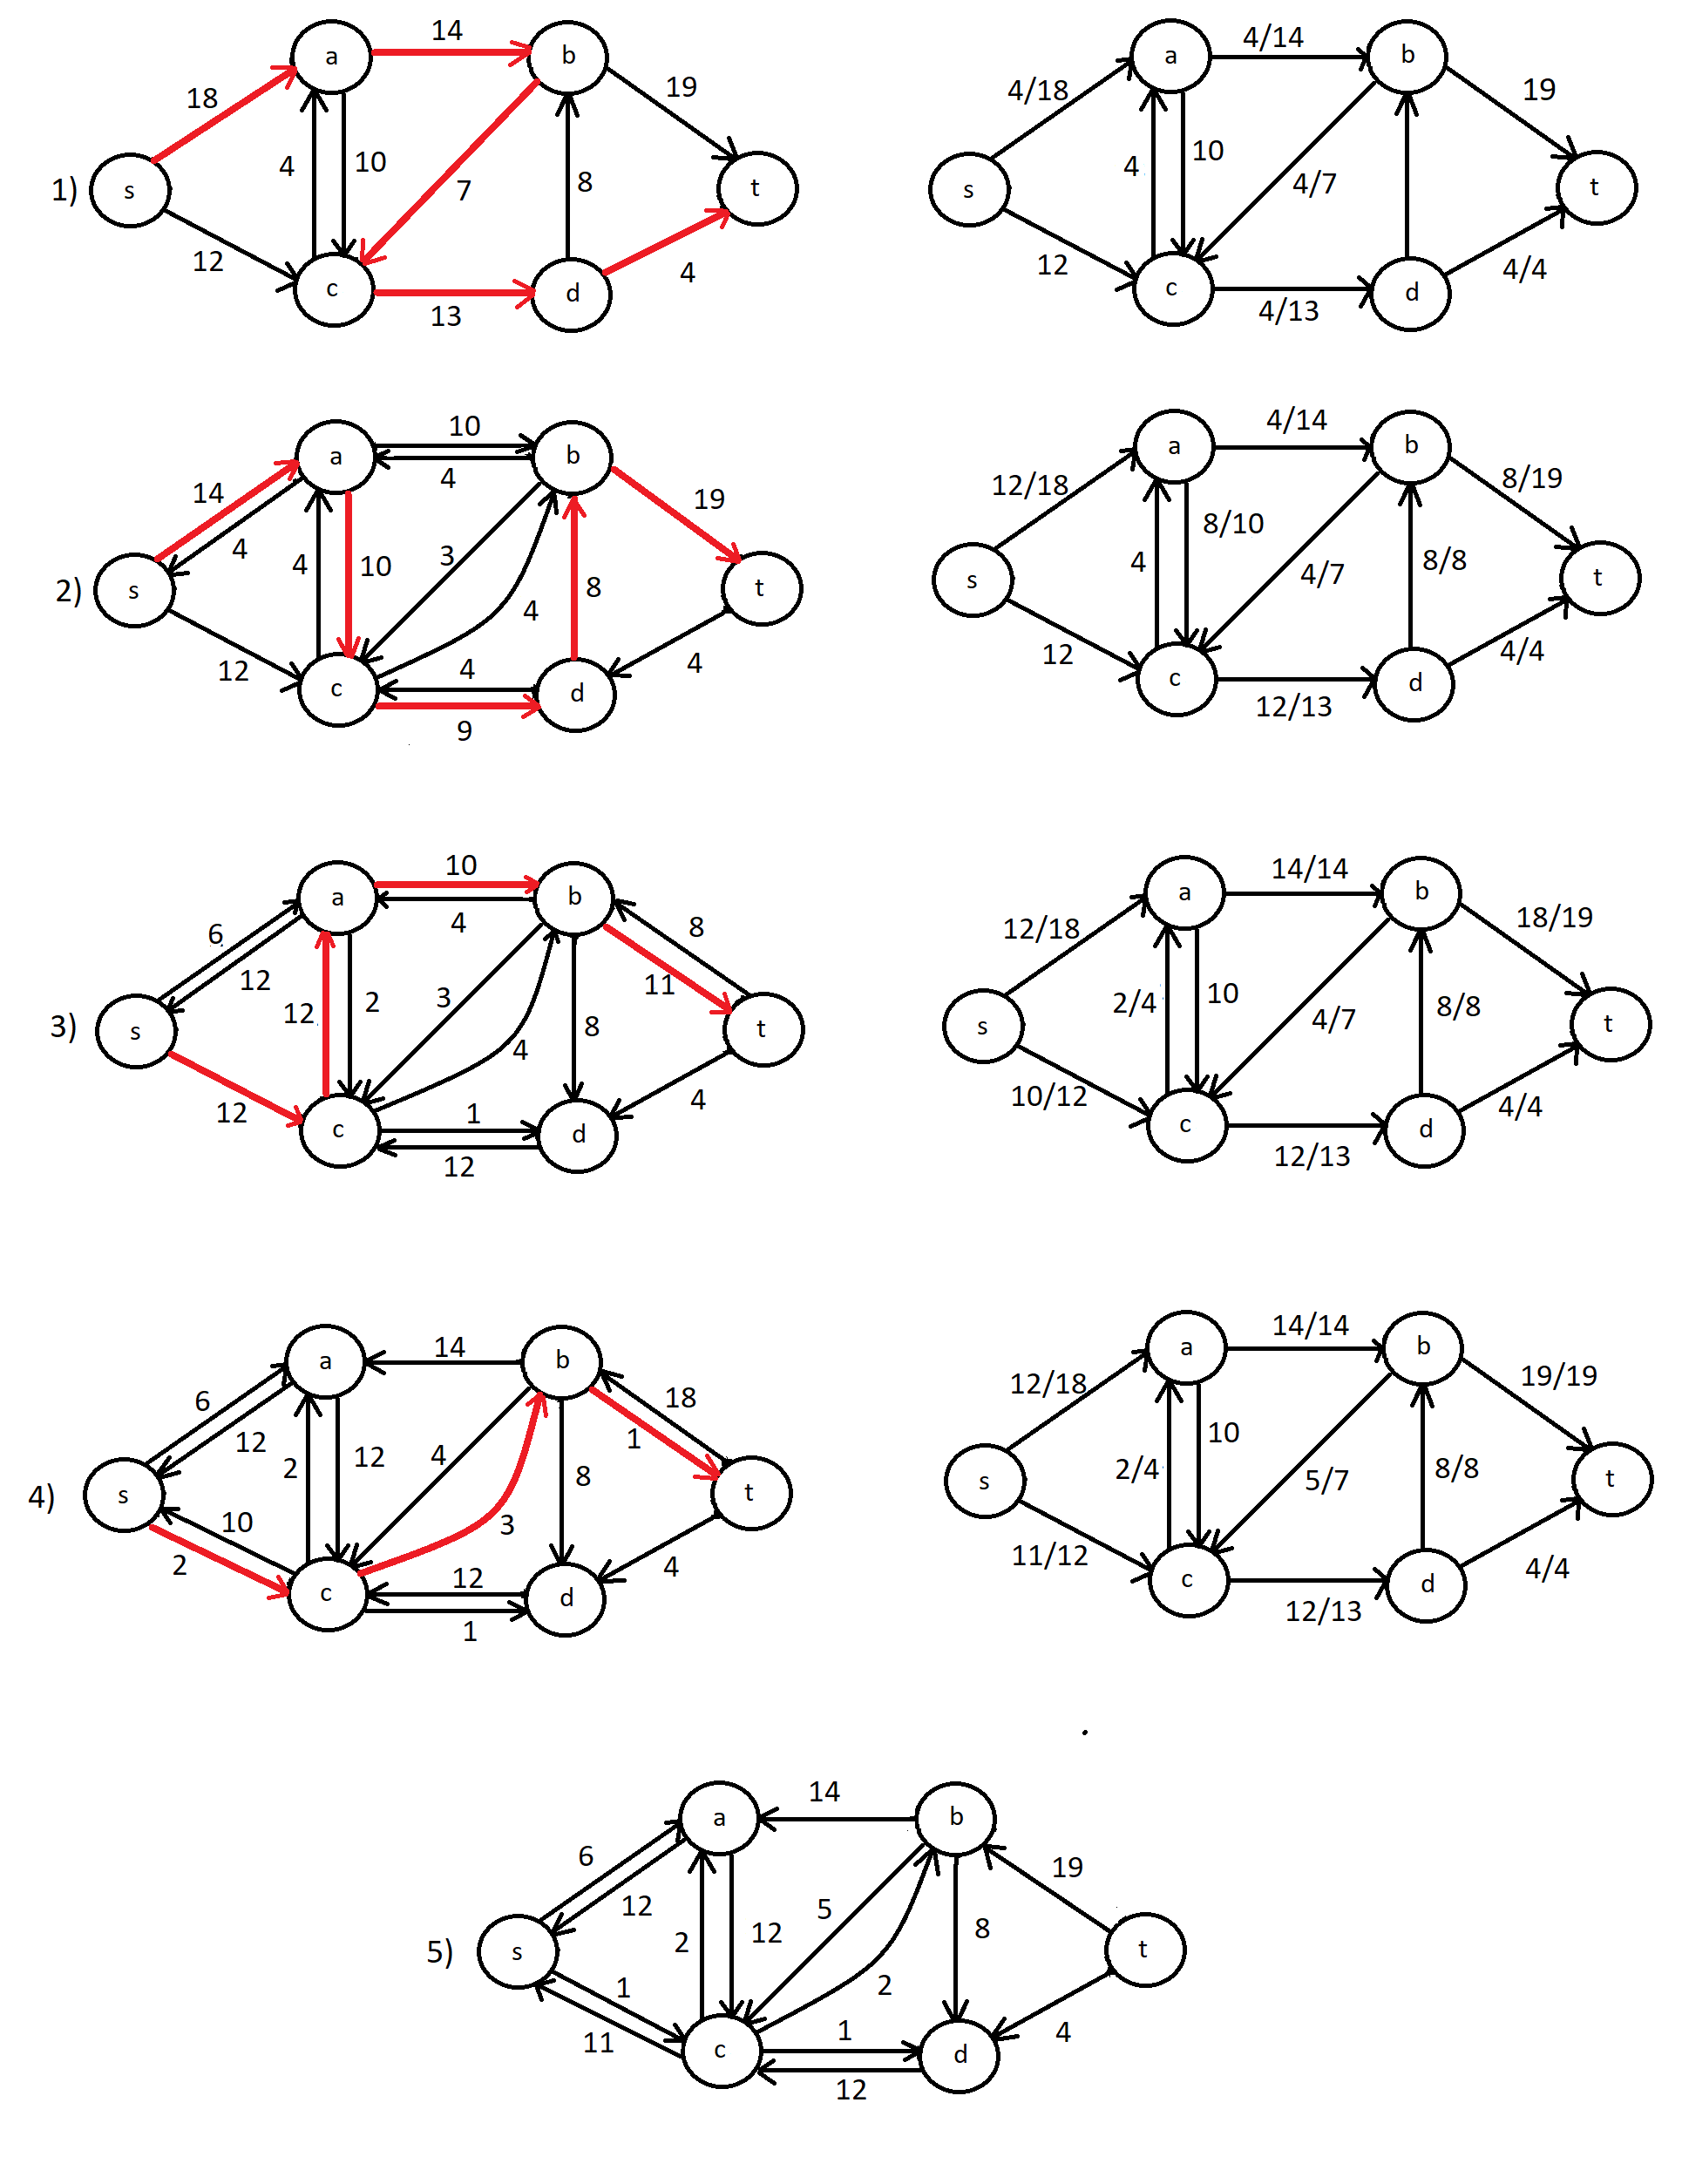
\includegraphics[width=13cm]{Ford-Fulkerson.png}
  	\caption{Exemplificarea algoritmului al lui For-Fulkerson. Re\c teaua reziduala \textbf{(1)} este re\c teaua de intrare $G$.\textbf{(1)-(4)} Itera\c ttiile succesive ale instruc\c tunii repetitive \textbf{while}. \^ In partea st\^ ang\u a se g\u asesc re\c telele reziduale $G_f$; drumurile de ameliorare $p$ sunt trasate cu ro\c su iar \^ in partea dreapt\u a se g\u asesc noile fluxuri $f$.\textbf{(5)} Re\c teaua rezidual\u a la ultimul test, aceasta nu mai co\c tine nici un drum de ameliorare, a\c sadar fluxul $f$ de la \textbf{(4)} este unul maxim.}
  \end{figure} 	
   	
   	
     \newpage
     \chapter{Aplica\c tie}
     
    \vspace{0.2cm} GPS-ul este un sitem de naviga\c tie  sub forma unui dispozitiv compact ata\c sat unei ma\c sini, avion sau a unei nave. GPS-ul prime\c ste informa\c tii de navigare \^ in timp real sub form\u a de coordonate din sateli\c ti.  \^ In ma\c sin\u a, GPS-ul \^ il ajut\u a pe \c sofer s\u a urmeze cea mai scurt\u a cale de la surs\u a la destina\c tie. GPS-ul de ast\u azi are caracteristici suplimentare cum ar fi: furnizarea de c\u ai alternattive la cea mai scurt\u a cale pentru a evita traficul sau construc\c tia drumurilor pe aceast\u a cale. Aceast\u a informa\c tie este important\u a deoarece cel mai scurt drum nu garanteaz\u a \^ intotdeauna sosirea \^ intr-un timp minim. Prin urmare, una sau dou\u a drumuri alternative sunt disponibile cu u\c surin\c t\u a \^ in dispozitiv.
    
    Astfel, un cet\u a\c tean str\u ain care nu cunoa\c ste harta ora\c sului, dore\c ste  s\u a ajung\u a \^ in timp util la o anumit\u a loca\c tie, folosind transportul public. Timpul alocat pentru a ajunge la destina\c tie este de preferat s\u a fie minim. Prin urmare, cu ajutorul unei aplica\c tii de navigare, acesta poate afla ce autobuze parcurg drumul dorit \^ intr-un interval minim de timp. Cet\u a\c teanul poate selecta loca\c tia curent\u a \c si destina\c tia pentru a afla rutele autobuzelor. F\u ac\^ and acest lucru, aplica\c tia genereaz\u a 3 drumuri optime \c si autobuzele care se deplaseaz\u a pe aceste drumuri. Dac\u a acesta afl\u a c\u a pe drumul optim generat de aplica\c tie sunt probleme ce \c tin de drum sau alte diverse motive care \^ impiedic\u a parcurgerea drumului, acesta are la dispozi\c tie alte dou\u a drumuri alternative pentru a ajunge la destina\c tie \^ intr-un timp minim.
     \subsection*{Implementare}
     
     
     Aplica\c tia GPS are la baz\u a algoritmului lui Dijkstra. Proiectul ilustreaz\u a un model GPS simplu
     pentru afi\c sarea a trei rute diferite \^ intre surs\u a și  destina\c tie. Proiectul
     produce versiunea offline a GPS-ului în care nu există date în timp real cu privire la coordonatele actuale ale
     \c soferului.
     
     Figura de mai jos (Figure 5.1) afi\c seaz\u a un simplu output pentru GPS. Rezultatul const\u a \^ in afi\c sarea unui graf cu noduri \c si muchii generate aleator \c si o fereastr\u a de vizualizare  \^ in care se g\u asesc informa\c tii de rutare. Programul afi\c seaz\u a deasemenea \c si alte informa\c tii despre autobuze cum ar fi: costul total, num\u arul de sta\c tii precum  \c si  drumul.
     
      Se creaz\u a mai \^ int\^ ai o copie a grafului $G$ pentru a se putea realiza opera\c tiile de reducere a grafului $G$. Primul drum este ob\c tinut din graful original $G$ cu 30 de noduri. Odat\u a ce drumul a fost ob\c tinut, muchiile  de-a lungul drumului sunt \^ indep\u artate pentru a reduce $G$ la $G'$. Algoritmul lui Dijkstra este aplicat din nou pentru $G'$ pentru a produce cel de-al doilea drum, care are un set de muchii diferit fa\c t\u a de primul. Respect\^ and algoritmul, muchiile celui de-al doilea autobuz sunt \^ indep\u artate pentru a reduce $G'$ la $G''$. Analog se aplic\u a acela\c si procedeu \c si pentru cel de-al treilea drum. Dup\u a ce sau generat toate cele 3 drumuri, copia grafului se va \^ inlocui cu originalul pentru a nu r\u am\^ ane eliminate muchiile de mai sus.
      
    \begin{figure}[!hbt]
	\centering
	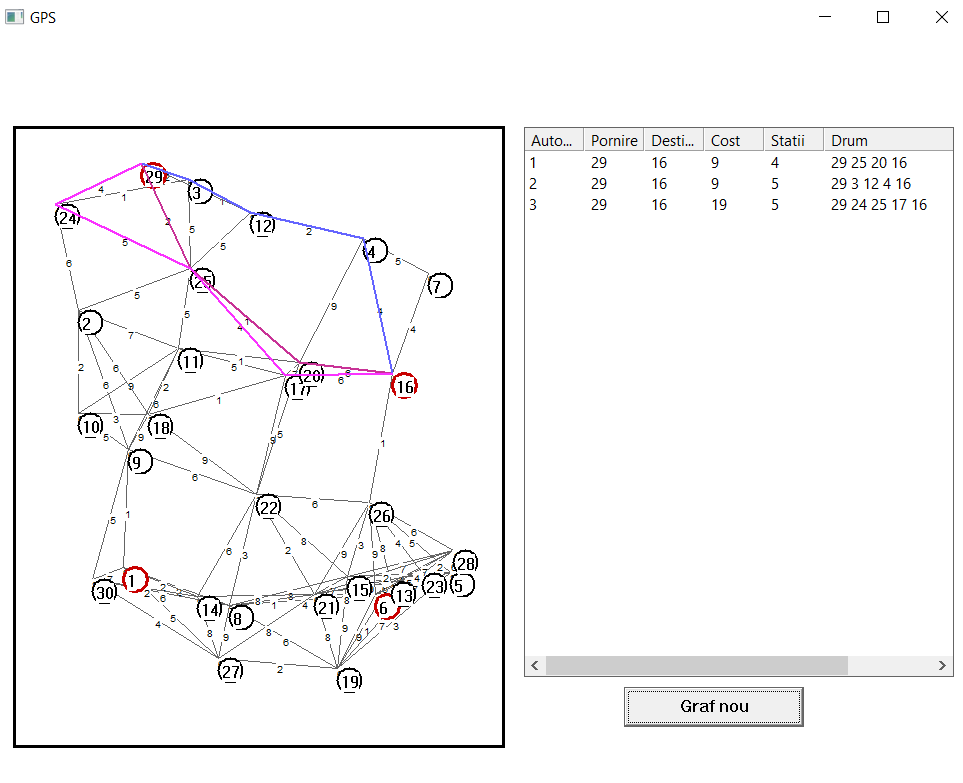
\includegraphics[width=12cm, height=7cm]{MiniGPS.png}
	\caption{Output-ul codului GPS care afi\c seaz\u a ruta a trei autobuze de la surs\u a la destina\c tie.} 
\end{figure} 
		 Sistemul GPS porne\c ste de la constructorul \textit{GPS()}, 
		care creeaz\u a o fereastr\u a \c si butonul \textit{Graf nou}. Aceast\u a func\c tie apeleaz\u a deasemenea func\c tiile 
		\textit{AfisareSetup()} \c si \textit{ResetareGraf()} care stabilesc  variabilele de afi\c sare comune \c si creeaz\u a graful. 
		\textit{ResetareGraf()} apeleaz\u a \textit{Initializare()} care creeaz\u a graful prin alocarea coordonatelor aleatorii la noduri \c si 
		costurile aleatorii la muchiile grafului. Graful ini\c tial este afi\c sat \c si reactualizat prin \textit{OnPaint()}.
		
		Evenimentul \textit{OnLButtonDown()} detecteaz\u a click-ul din st\^ anga mouse-ului a c\u arui pozi\c tie se afl\u a \^ in 
		Windows returnat de obiectul \textit{CPoint punct}. Valoarea obiectului este verificat\u a cu \textit{v[i].rct} folosind 
		\textit{PtInRect()} (aceast\u a func\c tie determin\u a dac\u a punctul specificat se afl\u a sau nu \^ in dreptunghi). Nodul surs\u a este identificat prin \textit{bFlag=1} iar destina\c tia prin \textit{bFlag=2}.
		
		\textit{Dijkstra()} calculeaz\u a cel mai scurt drum folosind algoritmul lui Dijkstra. Func\c tia este apelat\u a atunci c\^ and 
		nodul secund a fost selectat \^ in timp ce autobuzul de la surs\u a la nodul destina\c tie este desenat folosind \textit{Traseaz\u aDrum()}. 
		Odat\u a ce primul autobuz a fost finalizat, informa\c tiile sale sunt actualizate \c si afi\c sate \^ in fereastra de vizualizare. 
		Deasemenea, muchiile de la primul autobuz sunt \c sterse din graful original. \c Stergerea muchiilor este \^ indeplinit\u a de 
		\textit{Initialize()} \^ inlocuind valoarea muchiei cu 99.
		
		Cel de-al doilea autobuz este o repetare a primului autobuz prin referire la graful redus G'. Prin urmare, calculul pentru noul drum 
		dintre cele dou\u a noduri, va lua \^ in considerare faptul c\u a primul drum are noduri care nu sunt adiacente dealungul parcurgerii. 
		Programul calculeaz\u a noul drum care \^ in mod cert evit\u a primul drum. Similar, se aplic\u a aceea\c si metod\u a \c si pentru 
		drumul cu num\u arul 3.
   
        Variabile \c si obiecte importante din clasa $GPS$ \c si descrierea lor:
     \begin{center}
     	\begin{tabular}{ |p{3.1cm}|p{2cm}|p{6.1cm}|  }
    		
     		\hline
     		\multicolumn{3}{|c|}{\textbf{GPS}} \\
     		\hline
     		
     		\textbf{Variabile} & \textbf{Tipul} & \textbf{Descriere}\\
     		\hline
     		
     		$bgGraf$        & $CButton$   & Buton pentru generarea unui nou graf\vspace{0.1cm}  \\
     		\hline
     		$Autobuz[i].drum[k]$ & $int$       & Drumul $k$ \^ in autobuzul $i$\vspace{0.1cm} \\
     		\hline
     		$Autobuz[i].nNod$  & $int$       & Num\u arul de noduri prin care autobuzul $i$ a trecut \vspace{0.1cm}\\
     		\hline
     		$Autobuz[i].cTotal$      & $int$       & Costul total al autobuzului $i$\vspace{0.1cm}\\
     		\hline
     		$home$           & $CPonit$    & Col\c tul din st\^ anga sus al zonei grilei dreptunghiului \vspace{0.1cm}   \\
     		\hline
     		$v[i].cost[j]$     & $int$       & Costul dintre $(v_{i}, v_{j})$\vspace{0.1cm}\\
     		\hline
     		$v[i].sp[j]$     & $int$       & Drumul cel mai scurt dintre $(v_{i}, v_{j})$\vspace{0.1cm}\\
     		\hline
     		$v[i].rct$     & $CRect$       & Define\c ste un dreptunghi prin coordonatele col\c turilor din st\^ anga sus \c si dreapta jos\\
     		\hline
     		$NodPrecedent$             & $int$       & Nodul precedent al nodului curent\vspace{0.1cm}\\
     		\hline
     		$Sursa, \newline Destinatia$         & $int$       & Sursa \c si destina\c tia\vspace{0.1cm}\\
     		\hline
     		$nAutobuz$           & $int$       & Numarul de autobuze de succes\vspace{0.1cm}\\
     		\hline
     		$tabel$          & $CListCtrl$ & Tabela care afi\c seaz\u a autobuzele de succes\vspace{0.1cm}\\
     		\hline
     		$pAutobuz[i]$        & $CPen$      & Culoarea autobuzului i\vspace{0.1cm}\\
     		\hline
     		$Noduri$              & $constant$  & Num\u arul de noduri \^ in graf\vspace{0.1cm}\\
     		\hline
     		$LinkRange$      & $constant$  & Valoarea pragului intervalului pentru adiacen\c ta dintre dou\u anoduri din grafic\vspace{0.1cm}\\
     		\hline
     		$stareVarf[i]$          & $bool$      & Starea v\^ arfului $v_{i}$\vspace{0.1cm}\\
     		
     		\hline
     	\end{tabular}
     	
     \end{center}

     \newpage

     \begin{tikzpicture}[node distance=2cm]
\node (start) [startstop,xshift=-10em] {GPS};
\node (MiniGPSS)   [startstop, below of=start,xshift=-12em] {GPS.h};
\node (Source)  [startstop, right of=MiniGPSS,xshift=2.5em] {Proiect1.cpp};
\node (MiniGPS)  [process, below of=MiniGPSS,yshift=-1em,xshift=4em] {\hspace{1.5cm}$GPS()$ \newline Constructorul care creaz\u a fereastra principal\u a, butonul pentru crearea unui nou graf \c si ini\c tializarea unor variabile.};
\node (OnPaint)  [process, below of=MiniGPS,yshift=-3em] {\hspace{1.5cm}$OnPaint()$ \newline Deseneaz\u a afi\c sarea ini\c tial\u a care const\u a \^ in noduri \c si muchii din valorile atribuite \^ in $Initialize()$.};
\node (OnLButtonDown)  [process, below of=OnPaint,yshift=-3em] {\hspace{0.7cm}$OnLButtonDown()$ \newline Selecteaz\u a sursa \c si destina\c tia nodurilor din graf folosind mouse-ul.};
\node (ShowTable)  [process, below of=OnLButtonDown,yshift=-3em] {\hspace{1.3cm}$ArataTabel()$ \newline Creaz\u a  ferestra de vizualizare a listelor.};
\node (Dijkstra)  [process, below of=ShowTable,yshift=-3em] {\hspace{1.5cm}$Dijkstra()$ \newline Aplic\u a algoritmul Dijkstra pentru a crea cel mai scurt drum de la surs\u a la destina\c tie.};
\node (OnNewGraph)  [process, right of=MiniGPS,xshift=12em] {\hspace{1.5cm}$ResetareGraf()$ \newline Reseteaz\u a graful cu noi valori, deseneaz\u a graful \c si creaz\u a tabela pentru afi\c sarea autobuzelor.};
\node (GetCUN)  [process, right of=OnPaint,xshift=12em] {\hspace{1.5cm}$CMAN()$ \newline Calculeaz\u a cel mai apropiat nod nemarcat din nodul curent.};
\node (DrawNode)  [process, right of=OnLButtonDown,xshift=12em] {\hspace{1.5cm}$Traseaz\u aNod()$ \newline Deseneaz\u a un nod.};
\node (DrawPath)  [process, right of=ShowTable,xshift=12em] {\hspace{1.5cm}$Traseaz\u aDrum()$ \newline Deseneaz\u a cel mai scurt drum de la surs\u a la destina\c tie.};
\node (Initialize)  [process, right of=Dijkstra,xshift=12em] {\hspace{1.5cm}$Initializare()$ \newline Ini\c tializeaz\u a nodurile \c si muchiile a grafului \c si aloc\u a valori pentru autobuze. };
\node (DisplaySetup)  [process, below of=Initialize,yshift=-3em] {\hspace{1.5cm}$AfisareSetup()$ \newline Ini\c tializeaz\u a culorile \c si fonturile pentru afi\c sarea autobuzelor.};
\draw[arrow](MiniGPS)--(OnNewGraph);
\draw[arrow](OnPaint)--(GetCUN);
\draw[arrow](OnLButtonDown)--(DrawNode);
\draw[arrow](ShowTable)--(DrawPath);
\draw[arrow](Dijkstra)--(Initialize);
\draw[arrow](MiniGPSS)--(Source);
\draw[arrow](start)|-(DisplaySetup);
\draw[arrow](Source)-|(start);
\end{tikzpicture}
     \clearpage
	\begin{thebibliography}{99}
		\bibitem{Bondy}A. Bondy, U.S.R. Murty,\textit{ Graph theory}, Springer (2008), Graduate texts in mathematics 244.
		\bibitem{Cormen} T.H. Cormen, C.E. Leiserson, R.L. Rivest, \textit{Introducere în Algoritmi}, Computer Libris Agora, Cluj-Napoca,
		2000.\vspace{-0.15cm}
		\bibitem{AM}A.M.Mo\c sneagu, \textit{Structuri de date}, Note de curs, Ia\c si, 2019.
		\bibitem{Sedgewick}R. Sedgewick, \textit{Algorithms in C++ Part 5: Graph Algorithms (3rd Edition)}, Addison-Wesley Professional
		2008.



	\end{thebibliography}
\addcontentsline{toc}{chapter}{Bibliografie}
\end{document}